%!TEX TS-program = pdflatex
% dissertation.tex -- main dissertation file
%
% Wisconsin dissertation template
% Copyright (c) 2008-2009 William C. Benton.  All rights reserved.
%
% This program can redistributed and/or modified under the terms
% of the LaTeX Project Public License Distributed from CTAN
% archives in directory macros/latex/base/lppl.txt; either
% version 1 of the License, or (at your option) any later version.
%
% This program includes other software that is licensed under the
% terms of the LPPL and the Perl Artistic License; see README for details.
%
% You, the user, still hold the copyright to any document you produce
% with this software (like your dissertation).
%

%%% You'll want ``oneside'' for the deposit version, but probably not for any versions that don't need to meet the UW requirements
\documentclass[12pt,oneside,letterpaper]{memoir}

% preamble.tex -- packages to include
%
% Wisconsin dissertation template
% Copyright (c) 2008 William C. Benton.  All rights reserved.
%
% This program can redistributed and/or modified under the terms
% of the LaTeX Project Public License Distributed from CTAN
% archives in directory macros/latex/base/lppl.txt; either
% version 1 of the License, or (at your option) any later version.
%
% This program includes other software that is licensed under the
% terms of the LPPL and the Perl Artistic License; see README for details.
%
% You, the user, still hold the copyright to any document you produce
% with this software (like your dissertation).

%% You should use natbib
\IfFileExists{natbib.sty}{%
\usepackage[numbers,sort&compress]{natbib}%
}{}

%% You probably need appendix, if you want appendices
\IfFileExists{appendix.sty}{%
\usepackage{appendix}%
}{}

%% the spacing in memoir is weird, you'll need to use this
\DisemulatePackage{setspace}
\usepackage[onehalfspacing]{setspace}

%% List setup; the ``hanglist`` environment will allow you to have
%% nicely-typeset enumerated lists (i.e. with the numbers hanging in
%% the margins).  You need at least version 2.1 of enumitem.sty.  If
%% you don't have enumitem installed at all, hanglist will just be an
%% alias for enumerate.
\IfFileExists{enumitem.sty}{%
\usepackage[loadonly]{enumitem}[2007/06/30]%
\newlist{hanglist}{enumerate}{1}% 
\setlist[hanglist]{label=\arabic*.}%
\setlist[hanglist,1]{leftmargin=0pt}%
}{%
\newenvironment{hanglist}{\begin{enumerate}}{\end{enumerate}}%
}

%% Comment out any of these that you don't want
\usepackage{amssymb}
\usepackage{amsmath}
\usepackage{amsthm}
%\usepackage{theorem}
\usepackage{hyperref}

\IfFileExists{mathpartir.sty}{%
\usepackage{mathpartir}%
}{}

%%%%% LISTINGS package and setup
\IfFileExists{listings.sty}{%
\usepackage{listings}%
}{}

% MY includes
\usepackage{array}
\usepackage[usenames, dvipsnames]{color}
\usepackage[table,xcdraw]{xcolor}
\usepackage[labelfont=bf,justification=centering]{caption}
\usepackage{tabularx}
\usepackage{afterpage}
\usepackage{tikz}
\usetikzlibrary{shapes.geometric, arrows, shadows, decorations.markings}
\usepackage{subcaption}
\usepackage{multirow}
\newcommand{\rotate}[2]{\parbox[t]{2mm}{\rotatebox[origin=c]{#2}{#1}}}%
\usepackage{cleveref}

%% Get rid of ugly borders around PDF hyperlinks (e.g. for cross-references, bib entries, or URLs)
\hypersetup{pdfborder = 0 0 0}

%% You want microtype.
\IfFileExists{microtype.sty}{%
\usepackage[protrusion=true,expansion=true]{microtype}%
}{}

%\pagestyle{thesisdraft}

% Surround parts of graphics with box
\usepackage{boxedminipage}

%% booktabs (thx to Nate Rosenblum for bringing this beautiful package
%% to my attention)
\IfFileExists{booktabs.sty}{%
\usepackage{booktabs}%
}{}

% This is now the recommended way for checking for PDFLaTeX:
\usepackage{ifpdf}

%% Avoid ugly "Type 3" fonts
\usepackage{lmodern}
\usepackage[LY1]{fontenc}

%% Substitute your favorite serif and sans fonts here....
\IfFileExists{tgpagella.sty}{%
% TeX Gyre pagella, like Palatino
\usepackage{tgpagella}%
}{}

\usepackage[LY1]{eulervm}

% \ifpdf
% \usepackage[pdftex]{graphicx}
% \else
% \usepackage{graphicx}
% \fi

\usepackage{makeidx}
\makeindex

{\theoremstyle{plain}
\newtheorem{thm}{Theorem}[chapter]
\newtheorem{cor}[thm]{Corollary}
\newtheorem{define}[thm]{Definition}
\newtheorem{exmpl}[thm]{Example}
}
{\theoremstyle{remark}
\newtheorem{rmk}[thm]{Remark}
}

\newtheoremstyle{customsty1}
{3pt}%
{3pt}%
{}% --- body font
{}% --- indent amount
{\bfseries}% --- Theorem head font
{:}% --- Punctuation after head
{.5em}% --- space after head
{}% --- theorem head spec (can be left empty, meaning 'normal')

% Define 'newtheorems' that use ``customsty1''
{\theoremstyle{customsty1} 
}


%%% NB: the ``deposit'' chapter- and page- styles should conform to UW
%%% requirements.  If you are producing a pretty version of your
%%% dissertation for web use later, you will certainly want to make
%%% your own chapter and page styles.

\makechapterstyle{deposit}{%
  \renewcommand{\chapterheadstart}{}
  \renewcommand{\printchaptername}{}
  \renewcommand{\chapternamenum}{}
  \renewcommand{\printchapternum}{\parbox{2em}{\MakeLowercase{\Large\scshape\thechapter{}}} }
  \renewcommand{\afterchapternum}{}
  \renewcommand{\printchaptertitle}[1]{%
  \raggedright\Large\scshape\MakeLowercase{##1}}
  \renewcommand{\afterchaptertitle}{%
  \vskip\onelineskip \hrule\vskip\onelineskip}
}

\makepagestyle{deposit}
 
\makeatletter
 
\renewcommand{\chaptermark}[1]{\markboth{#1}{}}
\renewcommand{\sectionmark}[1]{\markboth{#1}{}}
 
\makeevenfoot{deposit}{}{}{}
\makeoddfoot{deposit}{}{}{}
\makeevenhead{deposit}{\thepage}{}{}
\makeoddhead{deposit}{}{}{\thepage}
\makeatother

%%% set up page numbering for chapter pages to satisfy UW requirements
%%% NB: You will want to delete until the ``SNIP'' mark if you are
%%% making a ``nice'' copy
\copypagestyle{chapter}{plain}
\makeoddfoot{chapter}{}{}{}
\makeevenhead{chapter}{\thepage}{}{}
\makeoddhead{chapter}{}{}{\thepage}
%%% SNIP

%%% bib nonsense
\makeatletter
\newenvironment{wb-bib}[1]{%
  \chapter*{references}
\ifnobibintoc\else 
\phantomsection 
\addcontentsline{toc}{chapter}{References} 
\fi 
\prebibhook
  \begin{bibitemlist}{#1}}{\end{bibitemlist}\postbibhook}

\AtBeginDocument{%
  \@ifpackageloaded{natbib}{% natbib is loaded
    \addtodef{\endthebibliography}{}{\vskip-\lastskip\postbibhook}
    \@ifpackagewith{natbib}{sectionbib}{% with sectionbib option
      \renewcommand{\bibsection}{\@memb@bsec}}%
      {\renewcommand{\bibsection}{\@memb@bchap}}}%
  {}
  \@ifpackagewith{chapterbib}{sectionbib}{%
    \renewcommand{\sectionbib}[2]{}
    \renewcommand{\bibsection}{\@memb@bsec}}{}
}
\makeatother

\input{includes/defs}
% thesisdefs.tex

% This is mostly adapted from withesis.cls.  The original copyright
% notice for withesis.cls follows, preceded by two percent signs (%%):

%% withesis.cls
%% LaTeX Style file for the University of Wisconsin-Madison Thesis Format
%% Adapted from the Purdue University Thesis Format
%% Originally by Dave Kraynie
%% Edits by Darrell McCauley
%% Adapted to UW-Madison format by Eric Benedict  (Noted with <EB>)
%% Updated to LaTeX2e by Eric Benedict 24 July 00
%% 
%%=============================================================================
%% Licensed under the Perl Artistic License.
%% see: http://www.ctan.org/tex-archive/help/Catalogue/licenses.artistic.html
%% for more info...
%%=============================================================================

% withesis.cls is available from CTAN.  The modifications to this file
% are also licensed under the Perl Artistic License.

% --wb, 2008

\makeatletter

\newcounter {tocpage}
\newcounter {lofpage}
\newcounter {lotpage}
\newcounter {listofheading}

\newcommand\@thesistitlemedskip{0.2in}
\newcommand\@thesistitlebigskip{0.6in}
\newcommand{\degree}[1]{\gdef\@degree{#1}}
\newcommand{\project}{\gdef\@doctype{A masters project report}}
\newcommand{\prelim}{\gdef\@doctype{A preliminary report}}
\newcommand{\thesis}{\gdef\@doctype{A thesis}}
\newcommand{\dissertation}{\gdef\@doctype{A dissertation}}
\newcommand{\department}[1]{\gdef\@department{(#1)}}

\newenvironment{titlepage}
 {\@restonecolfalse\if@twocolumn\@restonecoltrue\onecolumn
  \else \newpage \fi \thispagestyle{empty}
% \c@page\z@ -- deleted: count title page in thesis
}{\if@restonecol\twocolumn \else \newpage \fi}

\gdef\@degree{Master of Science}    %Default is PhD
\gdef\@doctype{A dissertation}         %Default is dissertation

\gdef\@department{(Electrical Engineering)} % Default is Electical Engineering
\gdef\@defensedate{01/01/2100}% Default is a long time from now.
\gdef\@committee{
  Suman Banerjee, Professor, Computer Sciences
  }

\renewcommand{\maketitle}{%
  \begin{titlepage}
%-----------------------------------------------------------------------------
% -- The thesis office doesn't like thanks on title page.  Put it in
% -- the acknowledgments.  This is here so you don't have to change
% -- your titlepage when converting from report style. -> from Purdue, but I
%        left it here since it seems compatible with UW-Madison, Eric
%-----------------------------------------------------------------------------
    \def\thanks##1{\typeout{Warning: `thanks' deleted from thesis titlepage.}}
    \let\footnotesize\small \let\footnoterule\relax \setcounter{page}{1}
    \begin{center}
      {\textbf{\expandafter\expandafter{\@title}}} \\[\@thesistitlebigskip]
       by \\[\@thesistitlemedskip]
      \@author \\[\@thesistitlebigskip]
      \@doctype\ submitted in partial fulfillment of \\
      the requirements for the degree of\\[\@thesistitlebigskip]
      \@degree \\[\@thesistitlemedskip]
      \@department \\[\@thesistitlebigskip]
      at the \\[\@thesistitlemedskip]
      UNIVERSITY OF WISCONSIN--MADISON\\[\@thesistitlemedskip]
      \@date
    \end{center}
    % \hspace*{-0.7in}Date of final oral examination: \@defensedate \\[\@thesistitlemedskip]
    \hspace*{-0.7in}The dissertation is approved by the following members of the 
    Final Committee:\\
    \@committee
  \end{titlepage}
  \setcounter{footnote}{0}
  \setcounter{page}{1} %title page is NOT counted
  \let\thanks\relax
  \let\maketitle\relax \let\degree\relax \let\project\relax \let\prelim\relax
  \let\department\relax
  \gdef\@thanks{}\gdef\@degree{}\gdef\@doctype{}
  \gdef\@department{}
  %\gdef\@author{}\gdef\@title{}
}


%=============================================================================
% ABSTRACT
%=============================================================================
% The abstract should begin with two single-spaced lines describing
% the author and title in a standard format.  After these lines comes
% the standard abstract.
%=============================================================================
\def\abstract{
  \chapter*{Abstract}
  \addcontentsline{toc}{chapter}{Abstract}
  \relax\markboth{Abstract}{Abstract}}
\def\endabstract{\par\newpage}


%=============================================================================
% UMI ABSTRACT
%=============================================================================
% The UMI abstract should begin with the author and title in a standard format.
% After the author comes the advisor and university. After these lines comes
% a bunch of double spaced text to make up the standard abstract.
% After the abstract, the advisor's approval signature follows.
% This page is not numbered and is delivered seperately to the thesis office.
%=============================================================================

\def\advisortitle#1{\gdef\@advisortitle{#1}}
\def\advisorname#1{\gdef\@advisorname{#1}}
\gdef\@advisortitle{Professor}
\gdef\@advisorname{Cheer E.\ Place}

\def\umiabstract{
             \thispagestyle{empty}
                  \addtocounter{page}{-1}
                \begin{center}
                  {\textbf{\expandafter\uppercase\expandafter{\@title}}}\\
                  \vspace{12pt}
                  \@author \\
                  \vspace{12pt}
                  Under the supervision of \@advisortitle\ \@advisorname\\
                  At the University of Wisconsin-Madison
                \end{center}
}

\def\endumiabstract{\vfill \hfill\@advisorname\par\newpage}


%============================================================================
% VERBATIMFILE
%============================================================================
% \verbatimfile{<filename>}    for verbatim inclusion of a file
% - Note that the precise layout of line breaks in this file is important!
% - added the \singlespace - EB
%============================================================================
\def\verbatimfile#1{\begingroup \singlespace
                    \@verbatim \frenchspacing \@vobeyspaces
                    \input#1 \endgroup
}


%=============================================================================
% SEPARATOR Pages
%   Creates a blank page with a text centered horizontally and vertically.
%   The page is neither counted nor numbered.
%   These pages are required in the thesis format before sections such
%   as appendices, vita, bibliography, etc.
%=============================================================================
\def\separatorpage#1{
  \newpage
  \thispagestyle{empty}
  \addtocounter{page}{-1}
  \null
  \vfil\vfil
  \begin{center}
    {\textbf{#1}}
  \end{center}
  \vfil\vfil
  \newpage}


%=============================================================================
% COPYRIGHTPAGE
%=============================================================================
% The copyright must do the following:
% - start a new page with no number
% - place the copyright text centered at the bottom.
%=============================================================================
\def\copyrightpage{
  \newpage
  \thispagestyle{empty}    % No page number
  \addtocounter{page}{-1}
  \chapter*{}            % Required for \vfill to work
  \begin{center}
   \vfill
   \copyright\ Copyright by \@author\ \@date\\
   All Rights Reserved
  \end{center}}


%=============================================================================
% GLOSSARY
%=============================================================================
% The glossary environment must do the following:
% - produce the table of contents entry for the glossary
% - start a new page with GLOSSARY centered two inches from the top
%=============================================================================
\def\glossary{
  \chapter*{GLOSSARY}
  \addcontentsline{toc}{chapter}{Glossary}}
\def\endglossary{\par\newpage}

%=============================================================================
% NOMENCLATURE
%=============================================================================
% The nomenclature environment must do the following:
% - produce the table of contents entry for the nomenclature section
% - start a new page with NOMENCLATURE centered two inches from the top
%=============================================================================
\def\nomenclature{\separatorpage{DISCARD THIS PAGE}
  \chapter*{Nomenclature}
  \addcontentsline{toc}{chapter}{NOMENCLATURE}}
\def\endnomenclature{\par\newpage}

%=============================================================================
% CONVENTIONS
%=============================================================================
% The conventions environment must do the following:
% - produce the table of contents entry for the nomenclature section
% - start a new page with CONVENTIONS centered two inches from the top
%=============================================================================
\def\conventions{\separatorpage{DISCARD THIS PAGE}
  \chapter*{Conventions}
  \addcontentsline{toc}{chapter}{CONVENTIONS}}
\def\endconventions{\par\newpage}


%=============================================================================
% COLOPHON
%=============================================================================
% The colophon environment must do the following:
% - produce the table of contents entry for the nomenclature section
% - start a new page with COLOPHON centered two inches from the top
%=============================================================================
\def\colophon{\separatorpage{DISCARD THIS PAGE}
  \chapter*{Colophon}
  \addcontentsline{toc}{chapter}{Colophon}}
\def\endcolophon{\par\newpage}

%=============================================================================
% LIST OF SYMBOLS
%=============================================================================
% The list of symbols environment must do the following:
% - produce the table of contents entry for the list of symbols section
% - start a new page with LIST OF SYMBOLS centered two inches from the top
%=============================================================================
\def\listofsymbols{\separatorpage{DISCARD THIS PAGE}
  \eject
  \chapter*{LIST OF SYMBOLS}
  \addcontentsline{toc}{chapter}{LIST OF SYMBOLS}}
\def\endlistofsymbols{\par\newpage}

%=============================================================================
% VITA
%=============================================================================
% The vita environment must do the following:
% - produce a separator page with the word vita centered
% - produce the table of contents entry for the vita
% - start a new page with VITA centered two inches from the top
%=============================================================================
\def\vita{
%  \separatorpage{VITA}         % UW doesn't require this EB
  \chapter*{VITA}
  \addcontentsline{toc}{chapter}{VITA}}
\def\endvita{\par\newpage}

%=============================================================================
% ACKNOWLEDGMENTS
%=============================================================================
% The acknowledgments environment must do the following:
% - start a new page with ACKNOWLEDGMENTS centered two inches from the top
%=============================================================================
\def\acks{
  \chapter*{Acknowledgments}
}
\def\endacks{\par\newpage}

%=============================================================================
% DEDICATION
%=============================================================================
% The dedication environment must do the following:
% - start a new page
% - center the text vertically
% - include the text in a center environment
%=============================================================================
\def\dedication{
  \newpage
  \null\vfil
  \begin{center}}
\def\enddedication{\end{center}\par\vfil\newpage}

%=============================================================================
% DATE
%=============================================================================
%\def\today{\ifcase\month\or
  %January\or February\or March\or April\or May\or June\or
  %July\or August\or September\or October\or November\or December\fi
  %\space\number\day, \number\year}
\newcount\@testday
\def\today{\@testday=\day
  \ifnum\@testday>30 \advance\@testday by -30
  \else\ifnum\@testday>20 \advance\@testday by -20
  \fi\fi
  \number\day\ \
  \ifcase\month\or
    January \or February \or March \or April \or May \or June \or
    July \or August \or September \or October \or November \or December
    \fi\ \number\year
}


%  Single counter for theorems and theorem-like environments:
\newtheorem{theorem}{Theorem}[chapter]
\newtheorem{assertion}[theorem]{Assertion}
\newtheorem{claim}[theorem]{Claim}
\newtheorem{conjecture}[theorem]{Conjecture}
\newtheorem{corollary}[theorem]{Corollary}
\newtheorem{definition}[theorem]{Definition}
\newtheorem{example}[theorem]{Example}
\newtheorem{figger}[theorem]{Figure}
\newtheorem{lemma}[theorem]{Lemma}
\newtheorem{prop}[theorem]{Proposition}
\newtheorem{remark}[theorem]{Remark}

%=============================================================================
% TABLE OF CONTENTS; LIST OF FIGURES; LIST OF TABLES
%=============================================================================
% In report style, \tableofcontents, \listoffigures, etc. are always
% set in single-column style.  @restonecol is used to keep track of
% whether we need to switch back to double column style after the toc.
%
% The only known problem now is that the first page with the new
% layout is too long.  The problem seems to be that the change to
% textheight doesn't take place on the first page.  Even if it's the
% first line in the table of contents macro.  Presumably the same
% problem also occurs in the lof and lot.
%
% I'm taking a shot at fixing the problem by dropping in a throw-away
% page between the change to the height parameters and the start of
% the chapter.  Isn't elegance wonderful?
%
%=============================================================================

% \def\@tableof#1#2#3#4#5{
% { % limit scope of following declarations!!
%   \@restonecolfalse\if@twocolumn\@restonecoltrue\onecolumn\fi
%   \addtolength{\textheight}{-40pt}       % -24-16
%   \addtolength{\majorheadskip}{-40pt}    % -24-16
%   \addtolength{\headheight}{52pt}        %  36+16
%   \addtolength{\headsep}{-12pt}          % -12
%   \separatorpage{DISCARD THIS PAGE}
%   \chapter*{#1}
%   #5
%   \relax\markboth{#1}{#1}
%   \hbox to \hsize{#2 \hfil Page}
%   \singlespace
%   \setcounter{#3}{0}
%   \setcounter{listofheading}{1}  % change from 0 to 1 by mccauley, 14may93
%   \def\@oddhead{\vbox to \headheight{\vspace{4pt}
%     \hbox to \hsize{\hfil\textrm{\thepage}} \vfil
%     \ifnum\value{#3}=1
%       \ifnum\value{listofheading}=2
%         \hbox to \hsize{Appendix\hfil} \vspace{4pt} \fi
%       \ifnum\value{listofheading}=1
%         \stepcounter{listofheading} \fi
%       \hbox to \hsize{#2 \hfil Page}
%     \else
%       \setcounter{#3}{1}
%     \fi}}
%   \def\@evenhead{\vbox to \headheight{\vspace{4pt}
%     \hbox to \hsize{\textrm{\thepage}\hfil} \vfil
%     \ifnum\value{#3}=1
%       \ifnum\value{listofheading}=2
%         \hbox to \hsize{Appendix\hfil} \vspace{4pt} \fi
%       \ifnum\value{listofheading}=1
%         \stepcounter{listofheading} \fi
%       \hbox to \hsize{#2 \hfil Page}
%     \else
%       \setcounter{#3}{1}
%     \fi}}
%   \@starttoc{#4}  \if@restonecol\twocolumn\fi
%   \newpage
% }}
% 
% \def\tableofcontents{\@tableof{TABLE OF CONTENTS}{}{tocpage}{toc}{}}
% 
% \def\listoffigures{
%   \@tableof{LIST OF FIGURES}{Figure}{lofpage}{lof}
%   {\protect\addcontentsline{toc}{chapter}{LIST OF FIGURES}}}
% 
% \def\listoftables{
%   \@tableof{LIST OF TABLES}{Table}{lotpage}{lot}
%   {\protect\addcontentsline{toc}{chapter}{LIST OF TABLES}}}

%=============================================================================
% BIBLIOGRAPHY
%=============================================================================
% The thebibliography environment executes the following commands:
%
%  o start a new 'chapter' with BIBLIOGRAPHY as the heading
%  o produce a separator page for the bibliography
%
%  \def\newblock{\hskip .11em plus .33em minus -.07em} --
%      Defines the `closed' format, where the blocks (major units of
%      information) of an entry run together.
%
%  \sloppy  -- Used because it's rather hard to do line breaks in
%      bibliographies,
%
%  \sfcode`\.=1000\relax --
%      Causes a `.' (period) not to produce an end-of-sentence space.
%=============================================================================
% \altbibtitle
%   The default title for the References chapter is ``LIST OF REFERENCES''
%   Since some people prefer ``BIBLIOGRAPHY'', the command
%   \altbibtitle has been added to change the chapter title.
%   This command does nothing more than change REFERENCES to BIBLIOGRAPHY
%============================================================================
\def\@bibchaptitle{Bibliography}
\def\altbibtitle{\def\@bibchaptitle{Bibliography}}
\def\thebibliography#1{
  %\separatorpage{\@bibchaptitle}
  \global\@bibpresenttrue
  \chapter*{\@bibchaptitle\markboth{\@bibchaptitle}{\@bibchaptitle}}
  \addcontentsline{toc}{chapter}{\@bibchaptitle}
  \vspace{0.375in}    % added to match 4 line requirement
  \interlinepenalty=10000 % added to prevent breaking of bib entries
  \singlespace\list
  {[\arabic{enumi}]}{\settowidth\labelwidth{[#1]}\leftmargin\labelwidth
    \advance\leftmargin\labelsep \usecounter{enumi}}
  \def\newblock{\hskip .11em plus .33em minus -.07em}
  \sloppy
  \sfcode`\.=1000\relax}
\let\endthebibliography=\endlist



\makeatother

\svnidlong{$LastChangedBy$}{$LastChangedRevision$}{$LastChangedDate$}{$HeadURL: http://freevariable.com/dissertation/branches/diss-template/dissertation.tex $} 

\clearpage\pagenumbering{roman}  % This makes the page numbers Roman (i, ii, etc)

\title{Some Applications of Machine Learning in Edge Computing and Mobility}
\author{Anantharaghavan Sridhar}
\department{Electrical Engineering}

\date{2016}


\newcommand{\CalciumIon}{\text{Ca}^{2+}}


\begin{document}

%%% Uncomment the following if your .bib contains references that you will not 
%%% explicitly cite, but that should be in the final bibliography:
% \nocite{*}

\ifpdf
\DeclareGraphicsExtensions{.pdf, .jpg, .tif}
\else
\DeclareGraphicsExtensions{.eps, .jpg}
\fi

\maketitle

%% Add \part declarations if you want, but it's not necessary
%\part{Preliminaries}

\svnidlong{$LastChangedBy$}{$LastChangedRevision$}{$LastChangedDate$}{$HeadURL: http://freevariable.com/dissertation/branches/diss-template/frontmatter/frontmatter.tex $}
\vcinfo{}

%%% SOME OF THIS CODE IS ADAPTED FROM THE VENERABLE withesis.cls

% COPYRIGHT PAGE
%  - To include a copyright page use \copyrightpage
\copyrightpage

% DEDICATION
\begin{dedication}
	\emph{Dedicated to my family, friends, my advisor and peers at UW-Madison.}
\end{dedication}

%% BEGIN PAGESTYLE

%%% You can pick a pagestyle if you want; see the memoir class
%%% documentation for more info.  The default ``deposit'' option meets
%%% the UW thesis typesetting requirements but is probably
%%% unsatisfactory for making a version of your dissertation that
%%% won't be deposited to the graduate school (e.g. for web or a nice
%%% printed copy)

\chapterstyle{deposit}
\pagestyle{deposit}


% ACKNOWLEDGMENTS
\begin{acks}
\begin{wbepi}{Albert Einstein}
Every one who is seriously involved in the pursuit of science becomes convinced that a spirit is manifest in the laws of the Universe-a spirit vastly superior to that of man, and one in the face of which we with our modest powers must feel humble.
\end{wbepi}

First and foremost, I would like to thank my advisor Professor Suman Banerjee for being an incredible mentor during my time at the University of Wisconsin-Madison.
 His vision and guidance have helped shape my research skills and have been the strongest force in showing me the wonders of academic life.


Next, I would like to thank my research mentor, Neil Klingensmith, without whose guidance I wouldn't have learnt half as much as I have.
 I cannot imagine a better grad school experience without the endless brainstorming discussions, support and encouragement from Neil.


Thank you to the Computer Sciences and Electrical Engineering departments at the University of Wisconsin-Madison for providing a wonderful research atmosphere.


Finally, thank you to my family, friends and loved ones. Thank you to my friends Bharadhwaj, Prashanth, Shruthi, Abisheik, Swami and many others for putting up with my quirkiness through 2.5 years of grad school.
 Thank you to Aparna for helping me find a balance between work and life.
 Thank you to my Mom and Dad for always having my back and giving me the confidence to pursue my interests.

\end{acks}

% CONTENTS, TABLES, FIGURES
\renewcommand{\printtoctitle}[1]{\chapter*{#1}}
\renewcommand{\printloftitle}[1]{\chapter*{#1}}
\renewcommand{\printlottitle}[1]{\chapter*{#1}}

\renewcommand{\tocmark}{}
\renewcommand{\lofmark}{}
\renewcommand{\lotmark}{}

\renewcommand{\tocheadstart}{}
\renewcommand{\lofheadstart}{}
\renewcommand{\lotheadstart}{}

\renewcommand{\aftertoctitle}{}
\renewcommand{\afterloftitle}{}
\renewcommand{\afterlottitle}{}

\renewcommand{\cftchapterfont}{\normalfont} 
\renewcommand{\cftsectionfont}{\itshape} 
\renewcommand{\cftchapterpagefont}{\normalfont} 
\renewcommand{\cftchapterpresnum}{\bfseries} 
\renewcommand{\cftchapterleader}{} 
\renewcommand{\cftsectionleader}{} 
\renewcommand{\cftchapterafterpnum}{\cftparfillskip} 
\renewcommand{\cftsectionafterpnum}{\cftparfillskip} 

% \captionnamefont{\small\sffamily} 
% \captiontitlefont{\small\sffamily} 

% \renewcommand{\contentsname}{contents}
% \renewcommand{\listfigurename}{list of figures}
% \renewcommand{\listtablename}{list of tables}

\tableofcontents

\clearpage
\listoftables

\clearpage
\listoffigures

\clearpage
% NOMENCLATURE
% \begin{conventions}
% % \begin{description}
% % \item{\makebox[0.75in][l]{term}
% %        \parbox[t]{5in}{definition\\}}
% % \end{description}
% \input{conventions}
% \end{conventions}

%% The UW graduate school no longer wants a UMI abstract page
%% Should you need one for some reason, uncomment the following
%% lines.  Thanks to Matt Fredrikson for reporting this!

% \advisorname{Gottlob Frege}
% \advisortitle{Professor}
% \begin{umiabstract}
%  
Recent advancement in Deep Learning for Image Classification and Perception tasks have contributed to incredible advancements in consumer technology.
 Devices such as Google Home, projects such as self-driving cars are now closer to reality than ever, thanks to the capacity of deep learning algorithms and research.
 However, the systems research community has been slower to catch up with the wave of deep learning, in the areas of edge computing and wireless systems.

The objective of this thesis is to expose the reader to some possible applications and ideas for applying machine learning and deep learning techniques in systems research.
 Particularly, the focus of this thesis is on edge computing, wireless and mobile systems where I believe there is large scope for defining new applications for machine learning research.

% \end{umiabstract}

\begin{abstract}
  
Recent advancement in Deep Learning for Image Classification and Perception tasks have contributed to incredible advancements in consumer technology.
 Devices such as Google Home, projects such as self-driving cars are now closer to reality than ever, thanks to the capacity of deep learning algorithms and research.
 However, the systems research community has been slower to catch up with the wave of deep learning, in the areas of edge computing and wireless systems.

The objective of this thesis is to expose the reader to some possible applications and ideas for applying machine learning and deep learning techniques in systems research.
 Particularly, the focus of this thesis is on edge computing, wireless and mobile systems where I believe there is large scope for defining new applications for machine learning research.

\end{abstract}

\clearpage\pagenumbering{arabic}

%%% END STUFF TAKEN FROM WITHESIS EXAMPLE FILE


%% Now include the tex files for each chapter, like so (I put these in separate dirs): 
\chapter{Introduction}

\cite{SPOCK} saves the galaxy.

\chapter{Water Hardness Detection in Building Water Supply}
\label{chap:water}

\section{Introduction}

Domestic and Industrial water supply contain dissolved minerals of varying concentration.
 The "hardness" of water \cite{WhatIsWaterHardness} is used to refer to a certain subset of dissolved minerals, specifically Calcium and Magnesium.
 In domestic water supply, the dissolved minerals contributing to hardness affect the longevity of appliances \cite{SoftenedWaterBenefitsStudy} while simulatenously increasing health risks to the occupants \cite{PotentialHealthImpactsOfHardWater} \cite{WaterHardnessOnCardiovascularDisease}.
 In industrial water supply, especially medical research labs, mandate extremely low hardness levels.
 Consequently, water softening solutions are sought to minimize the ill effects of water hardness.

A typical solution to the water hardness levels is to install water softeners in the consuming units (residential or industrial units).
 Water Softeners are a primary source of Sodium and Chloride ion pollution in fresh water sources.
 The pollution arises as a result of softener regeneration, which produces effluent water with exteremely high mineral concentration (extremely high water hardness).
 This effluent finds its way into water treatments facilities which face challenges in removing the dissolved minerals.

The regeneration process is triggered in the water softeners based on a threshold on the aggregate water flow through the softener since the last regeneration.
 This is referred to as the "reserve capacity algorithm".
 Since the regeneration process is blind to the actual hardness in the water, there are three possible cases:

\begin{enumerate}
\item \emph{Case 1:} The regeneration happens \textbf{after} the softener has depleted its capacity, allowing hard water to reach the consumers and appliances.
 This is undesirable.
\item \emph{Case 2:} The regeneration happens \textbf{before} the softener has depleted its capacity, resulting in higher regeneration frequency and increased softener effluent discharge to water treatment facilities.
 This is undesirable.
\item \emph{Case 3:} The regeneration happens at the \textbf{exact} time when the softener is close to depletion, achieving balance between frequent regenerations and hard water mitigation.
\end{enumerate}

Case 3 does not occur in commercial water softeners since the softeners are programmed pessimistically and favor frequent regenerations (Case 2) to minimize the risk of hard water reaching the consumer (Case 1).
 As a solution to this pessimism, the AWESOME system \cite{AWESOME} provides a mechanism to control the tradeoff between Case 1 and Case 2.
 The AWESOME \cite{AWESOME} system is an example of an Edge Computing platform where the computation and intelligence is decentralized by leveraging compute power at the "edge" of connectivity (e.g. using WiFi routers in the home).
 In the case of AWESOME, Machine Learning algorithms are deployed at the edge, using edge computing resources.
 There are two key Machine Learning challenges involved in the solution.

\paragraph{Water Hardness Detection:} The hardness is measured using Calcium ion ($\CalciumIon$) sensors at the output of the water softener.
 However, the sensors do not measure a clean, trivially recognizable hardness signal.
 The measurements exhibit several "false" hardness events, where the signal shares characteristics with a true hardness event.
 We built a Support Vector Machine to distinguish between the false hardness events and the true hardness events.
 When a true hardness event occurs, it is an indication of the depleted state of the water softener.

\paragraph{Water Flow and Hardness Forecasting:} The hardness is highly dependent on the water flow patterns of the building.
 Once it is possible to distinguish between true and false hardness events from the sensor signals, predicting the flow patterns of a building would allow to forecast the exact time of the hardness event ahead of time.
 This allows flexibility in better protecting the consumers and appliances (Case 1) while minimizing effluent discharge (Case 2).





\section{Water Hardness Detection}

The objective is to devise features and learn a Support Vector Machine (SVM) that is able to distinguish between true hardness events and false hardness events in the water at the output of the water softener.


\subsection{Feature Engineering}

The following features were chosen by empirical studies as being most "informative" towards this classification task.

\begin{enumerate}
\item \emph{Measured Hardness:} This is directly calculated from the output of the Calcium ion ($\CalciumIon$).
 The sensor output is a voltage value which is converted to the corresponding hardness measurement in grains per gallon \cite{WhatIsWaterHardness}.
\item \emph{Flow Rate:} Flow rate is the average rate of flow over a 2 minute interval (can be considered as instantaneous rate of flow considering that the dynamics of the system are extremely slow).
 In this case, the "instantaneous" flow has been chosen as a feature in order to make the algorithm independent of the cumulative flow, unlike the reserve capacity algorithm.
 The reserve capacity algorithm uses the cumulative flow or the number of days since last regeneration to trigger the next regeneration \cite{NSFSoftener}.
\item \emph{Temperature:} This is chosen as a feature because the output voltage of the Calcium ion ($\CalciumIon$) sensor was found to fluctuate with the ambient temperature.
\item \emph{Derivative of the voltage output of the Calcium Ion ($\CalciumIon$) sensor:} This is used to encode some characteristics of the shape of the hardness measurement transient.
\item \emph{Temperature compensated voltage output of the Calcium Ion ($\CalciumIon$) sensor:} The relationship between the temperature and the voltage output of the sensor is highly nonliner and difficult to characterize.
 This hand engineered feature was included as a simple compensation technique for temperature effects to help the SVM improve its classification accuracy.
 This approach is similar to using kernel functions.

\end{enumerate}

The features are also described in \ref{tab:features_hard_water}. An example trace of raw hardness data is shown in Figure \ref{fig:example_trace_water_hardness}.

\subsection{Data Collection and Learning}
\label{sec:water_hardness_learning}

The data was collected from multiple installations of the AWESOME \cite{AWESOME} system over several months (with at least 2 instances of true hardness events from each installation).
 \footnote{The training was done after the appropriate pre-preprocessing using the \texttt{scikit-learn} Python library.}

SVM is a supervised learning algorithms, meaning that it requires a training phase in which input data labeled with ground truth is fed to the algorithm.
 When constructing the training sets for SVM, each feature vector with ground truth.
 I developed a web-based training tool for time-series data that allows for crowdsourced labeling.
 A screenshot of this tool is shown in in Figure \ref{fig:hardnesslabelingtool}.
 This training tool was used to directly generate data sets for SVM training.

This labeling process is subjective because the water hardness --- concentration of Calcium and Magnesium ions --- is a real number which must be converted to a binary value (0 or 1).
 So to label training data, a \textbf{training threshold} must be applied, below which water is considered to be soft (0), and above which it is considered to be hard (1).
 The threshold applied will affect the SVM's ability to distinguish between soft and hard water.
 If the training threshold is too low, the algorithm may classify all unknown inputs as hard (false positives).
 If the training threshold is too high, all hardness events may be ignored (false negatives).
 The objective is to produce training sets that will identify filtration medium depletion early (before the outgoing water has become too hard) while rejecting noise.
 This is discussed further in Section \ref{sec:water_hardness_evaluation}.

\begin{figure}[!t]
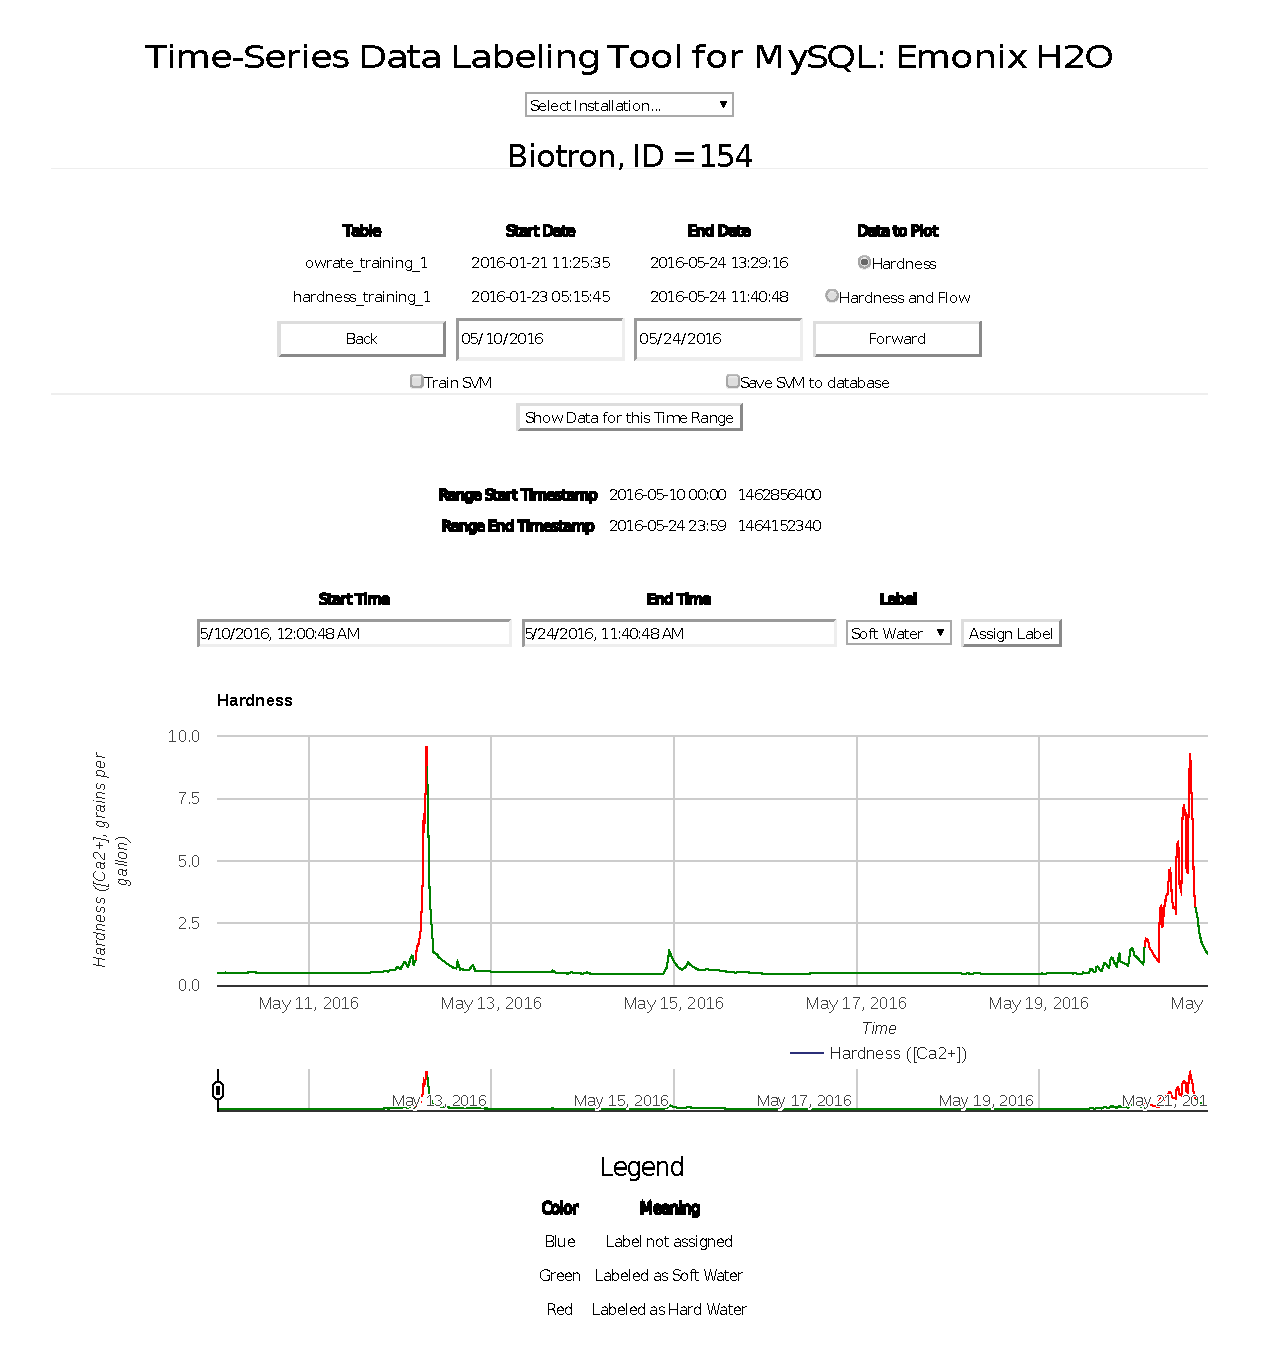
\includegraphics[width=\textwidth]{water/hardnesslabelingtool2.pdf}
\caption{Screenshot of Time-series data labeling tool developed for Water Hardness Labeling}
\label{fig:hardnesslabelingtool}
\end{figure}

\begin{table}
\centering
    \begin{tabularx}{\textwidth}{l || X || X }
    \textbf{Feature} & \textbf{Formula} & \textbf{Units} \\
    \hline
    ISE Output &  $[\CalciumIon] = e^{k (V - a)}$ & $[grains/gallon]$ \\
    Flow Rate &  $f$ & $[gal/minute]$ \\
    Temperature & $T$ & $[^\circ C]$ \\
    Derivative of ISE Output & $\frac{d [\CalciumIon]}{dt}$ & $[grains/gallon/minute]$ \\
    Normalized ISE Output & $[\CalciumIon] \left(  1 - e^{-k f / T}\right) $ & $[grains/gallon]$ \\
    \end{tabularx}
\caption{Description of hand-engineered features used to detect hard water}
\label{tab:features_hard_water}
\end{table}

\begin{figure}
\centering
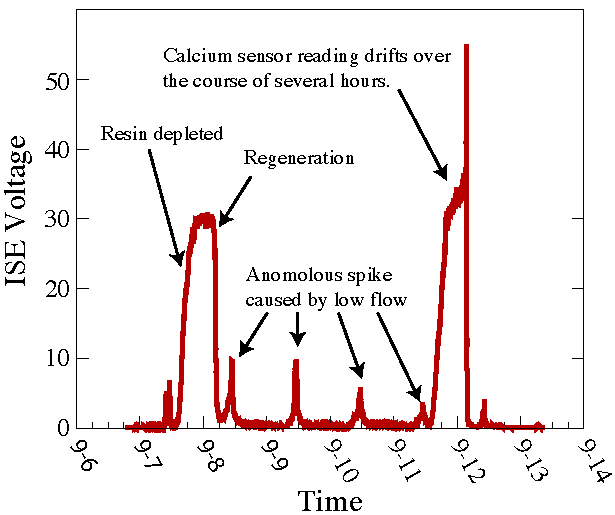
\includegraphics{water/hardness-snapshot.pdf}
\caption{Example trace of raw water hardness data showing both true and false hardness events}
\label{fig:example_trace_water_hardness}
\end{figure}

\subsection{Evaluation}
\label{sec:water_hardness_evaluation}

\begin{enumerate}
\item How quickly can the SVM identify depletion of the water softener (true hardness event)?
\item How resistant is each algorithm to anomalous sensor inputs (noise)?
\end{enumerate}

The answer to the first question will give insight that is similar to a false-negative rate.
 An important figure of merit is the amount of time it takes the system to detect water softener resin depletion.
 The earlier the detection happens, the lesser the impact of hard water on the residence or industrial facility.
 The longer it takes the SVM to detect that the resin has been depleted, the harder the water that is produced by the softener, potentially endangering building systems.

The answer to the second question will tell us the false positive rate.
 When the SVM produces a false positive, it regenerates the softener unnecessarily, wasting salt.

To identify filtration medium depletion, it will be necessary to allow the medium to deplete and start producing hard water.
 The goal is to minimize the amount of hard water that needs to be produced before the SVM can identify that the medium is depleted.
 If too much hard water is supplied to a building before initiating a regeneration, the water heater and other building systems could suffer damage.


In order to make the SVM detect hard water as early as possible, the training threshold (described in Section \ref{sec:water_hardness_learning}) is manually adjusted based on empirical performance feedback.
 The lower the training threshold is set, the earlier the SVM will be able to detect filtration medium depletion.
 Figure \ref{fig:hardnessresults} shows a plot of the average outgoing water hardness level at which the algorithm can detect medium depletion for several different training thresholds.
 The figure presentes a comparison of the hardness detection level between simple thresholding and the SVM (simple thresholding has a high false positive rate, as evident from Figure \ref{fig:example_trace_water_hardness}).
 The y-axis gives the average water hardness required for each algorithm to identify a filtration medium depletion.
 To be practical, the detection level should be below five grains per gallon because allowing the hardness to get any higher would damage building systems.


At low training thresholds, the learning algorithms tend to produce more false positives.
 Figure \ref{fig:falsepositives} shows the false positive rates on the y-axis with the algorithm on the x-axis.
 To strike a balance between minimizing false positives and minimizing the hardness detection level, it is best to train the learning algorithms to identify depletion at three grains hardness.


The receiver operating curve (ROC) shown in Figure \ref{fig:roc} shows the tradeoff between false positives and true positives for SVM and thresholding.
 On the y-axis, true positives are plotted as a function of false positives.
 The SVM performs much better than thresholding because we only need to increase the proportion of false positives to 30\% in order to achieve 90\% true positive detection.



\begin{figure}[t]
\centering
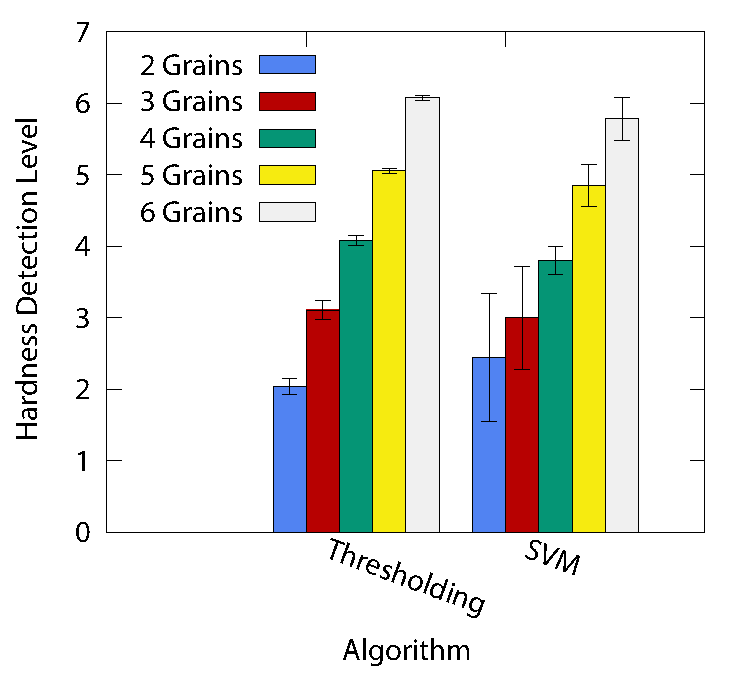
\includegraphics{water/hardnessresults.pdf}
\caption{The water hardness level of detection for five different training levels.}
\label{fig:hardnessresults}
\end{figure}


\begin{figure}[t]
\centering
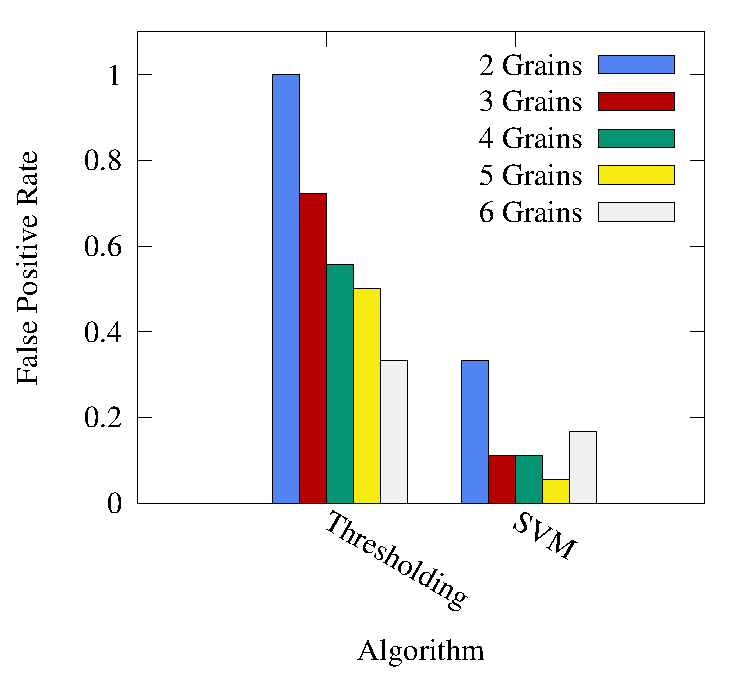
\includegraphics{water/hardnessfalsepositives.pdf}
\caption{False positive rates for the water hardness detection learning algorithm, tested with five different training thresholds.}
\label{fig:falsepositives}
\end{figure}

\begin{figure}[t]
\centering
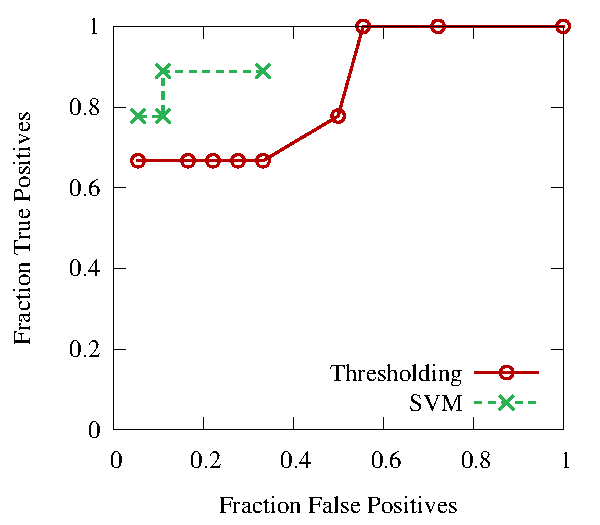
\includegraphics{water/hardnessroc.pdf}
\caption{Receiver operating curve for the water hardness detection learning algorithm.}
\label{fig:roc}
\end{figure}


\section{Water Flow and Hardness Forecasting}

The objective is to forecast water flow and water hardness at the output of the water softener based on historical patterns.
 Forecasting the water flow based on historical patterns is equivalent to modeling the water usage behaviour of a building (residential or industrial).
 Forecasting the water hardness based on historical patterns is equivalent to modeling the physics of the water softener itself and its depletion characteristics.

\subsection{Water Flow Forecasting}

A statistical analysis of water flow patterns in various buildings indicate that the flowrate function is not a stationary process over long time periods.
 \footnote{A stationary process is one whose statistical properties do not change as a function of time. In other words, $X_t$ is stationary iff $F_X (x_{t_1} ... x_{t_k}) = F_X (x_{t_{1+l}} ... x_{t_{k+l}})$}
 This finding makes sense because activities in a building will likely follow daily circadian fluctuations.
 At 4 AM, when most residents are asleep, the histogram indicates that the recorded flow rates are mostly zero.
 Flow rates increase around 8 AM when residents wake up to go to class.
 At noon, flowrates increase further because lunch is served in the building's cafeteria.
 Since the distribution of water flow rates changes during the course of the day, it is reasonable to conclude that the process is nonstationary.

Since the flowrate signal is nonstationary, the modeling approach should deal with data that has time-varying distribution.
 An autoregressive model is a commonly used tool to forecast stationary processes \cite{oppenheim2010discrete}.
 Here, the autoregressive approach is adapted to work with a nonstationary process, leveraging continuous data measurements.

The flowrate signal tends to be bursty --- it tends to be high for a short time when a fixture is turned on and low when the fixture is off.
 In large buildings, that burstiness is contributed by hundreds of fixtures, each contributing to a noisy signal with a lot of high-frequency components.
 To deal with such a large magnitude of high frequency components, an extremely high order of autoregressive model will be required, which makes the modeling infeasible.
 Instead of forecasting the raw flowrate, forecasting the cumulative flow is a reasonable compromise (equivalent to passing the flowrate signal through an integrator).
 The resulting autoregressive model will have poor accuracy in forecasting instantaneous flowrate.
 However, this cumulative flow signal is a more useful metric anyway --- the cumulative flow is the more important metric for understanding softener depletion.

The autoregressive model then predicts the cumulative flow used by the building on a minute-by-minute basis, 24 hours into the future.
 The results of the predictions made by the autoregressive model will be presented in Section \ref{sec:eval-forecasting}.

\subsection{Water Hardness Forecasting}

In addition to forecasting flow, it is also beneficial to predict water hardness readings, since it will be the better indicator of softener depletion.
 If the water softener's filtration medium will not be depleted in the near future according to predictions (i.e. water will not be hard), there is no point in regenerating the water softener.


Similar to the flow forecasting technique, a vector-state autoregressive model is used to predict future cumulative flow and hardness together.
 Unlike the flow rate signal, the hardness signal is sparse.
 Most of the hardness readings are zero or nearly zero---this is expected because when the water softener is working properly, it removes all hardness from the water.
 It is only when the water softener's filtration medium depletes that nonzero hardness is observed.
 The sparse nature of the hardness readings and the inherent nonlinearity of the hardness with respect to the cumulative water flow through the softener poses a challenge for learning linear, stationary models, such as, autoregressive models.


To account for the inherent nonlinearity so described, two operating point models are used (for low/high cumulative flow since the last regeneration).
 This is justified on the basis that the nonlinearity of the hardness measurement only manifests itself in the high flow region.
 A parallel can be drawn between this approach and the general practice of linearizing nonlinear systems near typical operating points for the design of closed-loop controllers.
 Since the hardness measurements depend on the cumulative flow through the softener since the last regeneration, in addition to the history of the hardness measurements themselves, the model can be represented in the following discrete-time state space notation ($flow(\dots)$ refers to the cumulative flow since the last regeneration):

\begin{gather}
X(k+1) = \begin{bmatrix}
A_{\text{flow-flow}} & 0_{\text{flow-hardness}} \\ 
C_{\text{hardness-flow}} & D_{\text{hardness-hardness}}
\end{bmatrix} X(k) \\
X(k) = \begin{bmatrix}
\text{flow}(k) \\
\dots \\
\text{flow}(k-20) \\
\text{hardness}(k) \\
\dots \\
\text{hardness}(k-20)
\end{bmatrix}
\end{gather}

$A_{\text{flow-flow}}$ captures the nature of the water usage by the residents of the building.
 Since this quantification is subject to rapid, unpredictable changes (nonstationarity), the forecasting model is learnt online after each regeneration cycle thereby using the most recent water usage patterns for the forecasting, eliminating bias due to historical data and addressing the nonstationary nature (resets due to regenerations).
 
 
The dependence of hardness measurements on their own history and the flow is quantified by the coefficients matrices of the mode $C_{\text{hardness-flow}}$ and $D_{\text{hardness-hardness}}$.
 The model so described is learned from recorded data for two operating regions (low/high cumulative flow since the last regeneration).
 When the actual forecasting is done, one of the models is chosen based on the flow since the last regeneration at the time of forecasting.

\subsection{Evaluating Forecasting Performance}
\label{sec:eval-forecasting}



\begin{figure*}[!th]
\centering
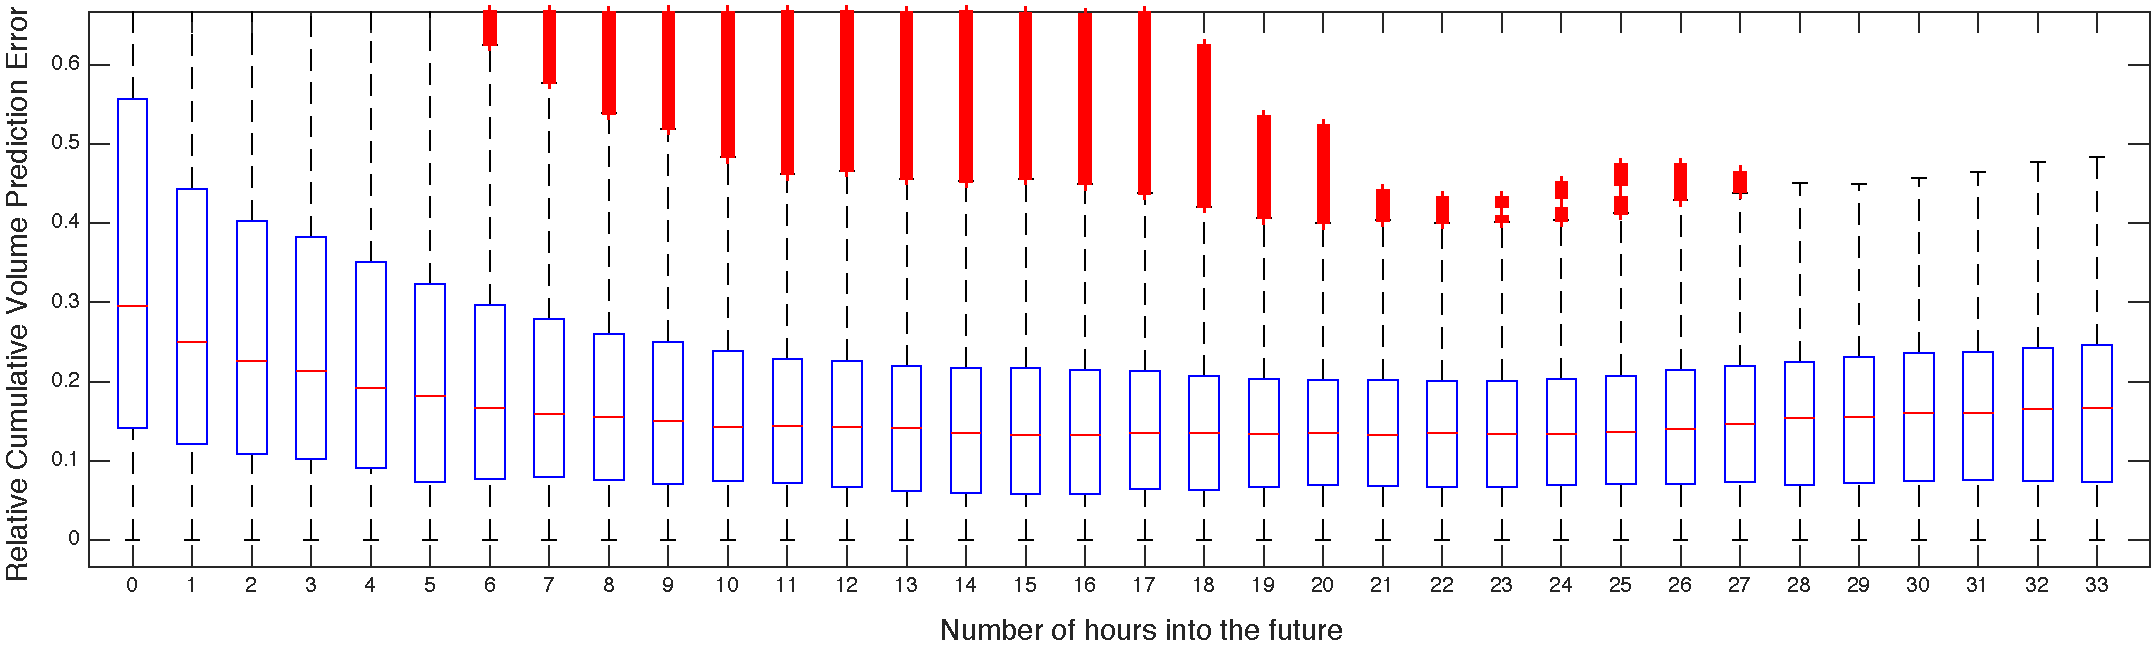
\includegraphics[width=\textwidth]{water/rel_cum_vol_pred_err.pdf}
\caption{Relative prediction error of cumulative water flow (y-axis) as a function of the forecast horizon (x-axis).}
\label{fig:cum_vol_pred_err}
\end{figure*}

\begin{figure*}[!th]
\centering
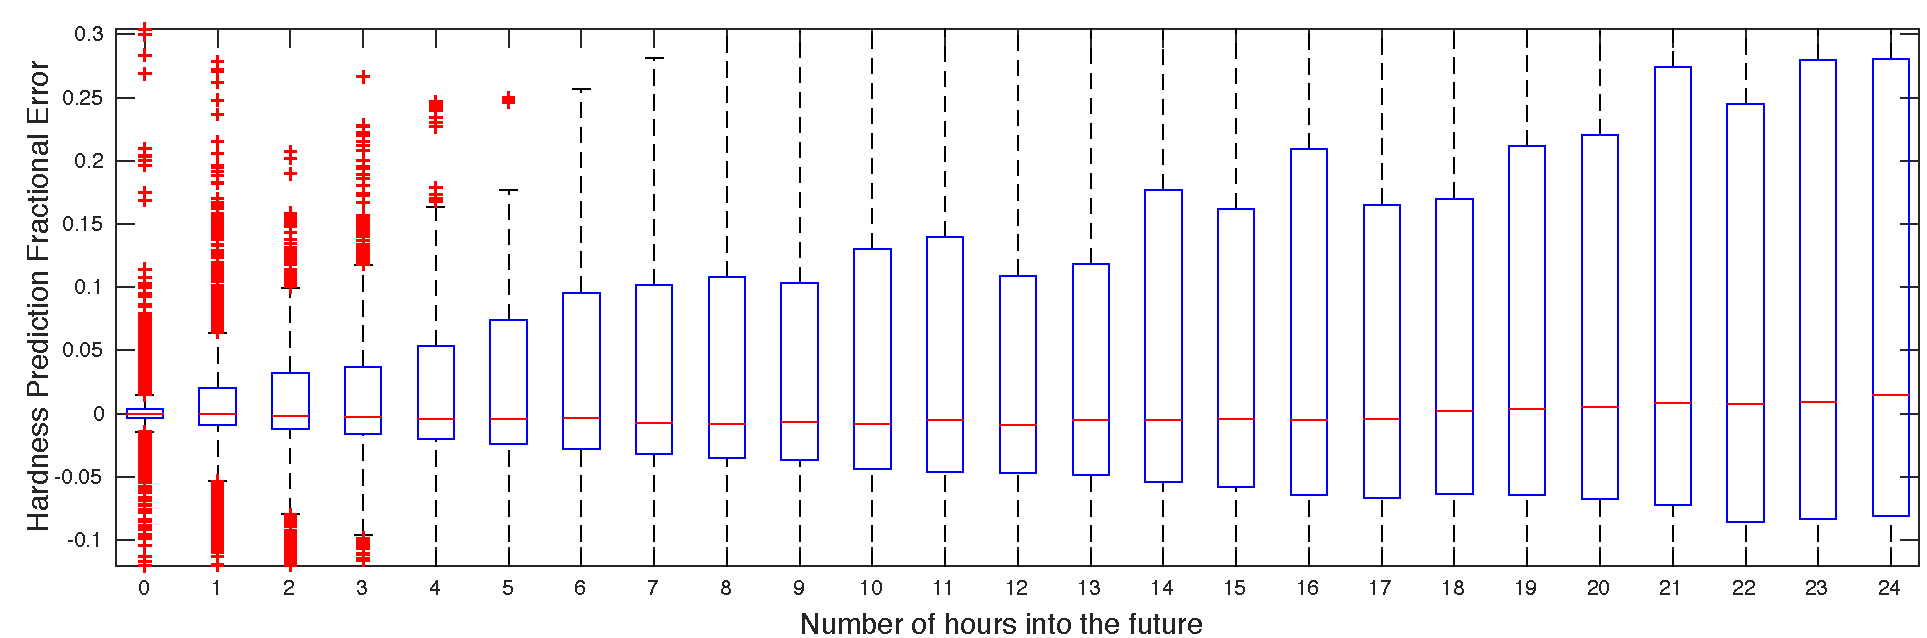
\includegraphics[width=\textwidth]{water/rel_hardness_pred_error_154.pdf}
\caption{Relative prediction error of water hardness (y-axis) as a function of the forecast horizon (x-axis).}
\label{fig:rel_hardness_pred_error_154}
\end{figure*}

\begin{figure}[!th]
\centering
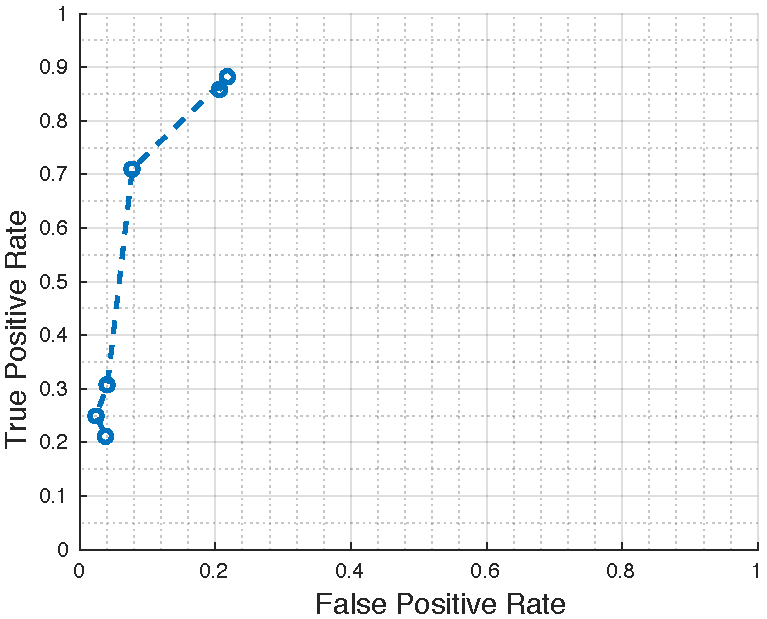
\includegraphics[width=\textwidth]{water/ROC_154.pdf}
\caption{Receiver operating characteristic for water hardness forecasting.}
\label{fig:forecastingroc}
\end{figure}

Relative prediction error is defined as

\begin{equation*}
e_{p_r}(h) = \left| \frac{p(t-h)-s(t-h)}{s(t-h)} \right|
\end{equation*}

where $h$ is the number of hours in advance the algorithm is predicting, $p(t)$ is the prediction as a function of time, and $s(t)$ is the actual measured sensor value as a function of time.
 Computations of relative prediction error for cumulative flow are shown in Figure \ref{fig:cum_vol_pred_err}.
 Computations of relative prediction error for instantaneous flow are shown in Figure \ref{fig:inst_flow_pred_err}.

Relative prediction error for cumulative flow is on average below 30\% and decreases for longer time horizons.
 The instantaneous flow signal tends to be very bursty---as fixtures turn on and turn off in the building, water flow starts and stops sporadically.
 If these bursts do not arrive at the exact moments that the algorithm expects them to, but instead arrive several minutes before or after, then the near-term cumulative flow error will be higher.
 As long as the bursts of flow eventually arrive, the long-term cumulative flow is low because it captures all the flow that has happened over a long period of time, and the errors in the prediction cancel each other out.

The hardness forecasting algorithm is intended to predict whether or not water samples will read hard in the next 24-hour time horizon.
 Since our water hardness sensor readings are sparse---long stretches of zero readings followed by short periods of hard water readings---the objective is to predict not only the exact value of the hardness sensor readings but also the presence or absence of hard water.
 If, during a forecasting horizon, the hardness value is not predicted accuractely but the presence or absence of a hard water event is correctly identified, then the algorithm has largely achieved its goal.

A plot of the relative errors in hardness prediction is shown in Figure \ref{fig:rel_hardness_pred_error_154}.
 On average, the relative prediction errors are close to zero for time horizons up to 24-hours in the future.
 The variance, however, increases for predictions made further into the future.


A receiver operating curve for the hardness forecasting algorithm is shown in Figure \ref{fig:forecastingroc}.
 The ROC was generated by varying the threshold at which water is classified as being hard---higher thresholds resulted in a higher false positive rate.


\section{Conclusion}


In this chapter, I describe techniques to classify water hardness based on ion concentration sensors to determine the state of water softener depletion.
 In addition, I also describe techniques to adapt commonly used autoregressive models to nonstationary, nonlinear processes with a known nonlinearity (hard resets, sudden water hardness events).
 The adaptation is required to keep the order of the autoregressive model low, which in turn keeps learning and forecasting computationally light.

\chapter{Wireless Spectrum Estimation using Sparse Measurements}

\chapter{Privacy-sensitive Acoustic Perception for Mobile Devices}
\label{chap:sound}

\section{Introduction}

Speech enabled technology is an increasingly popular element in consumer devices, as seen in Smartphones, Home Assistants etc.
 To provide speech enabled features, devices rely on listening to the ambient raw audio stream for keyword spotting.
 Applications listening to raw audio pose serious questions about conversational privacy and personal security for the end-user \cite{alwaysListening}.
 As an attempt to protect privacy, the speech enabled features have been restricted only to "native" applications written by the device manufacturer.


In this chapter, I present a solution to this problem in two phases.
 I discuss audio obfuscation techniques and examine the trade-off between privacy and keyword spotting performance.
 I also identify the best solution within our framework that maximizes both privacy and keyword spotting performance.
 I present performance results in the field from an Android application (\texttt{dBHound Keyphrase}).
 I also support my argument with human level cognition performance on obfuscated audio.
 Using this approach allows the entire suite of applications on a consumer device to provide keyword-enabled services while maintaining user privacy.
 This is achieved by openly broadcasting the obfuscated audio to the applications on the device.
 Since most user interaction with applications can be decomposed into keywords, I envision that this approach will lead to comprehensive speech-enabled services while maximizing end-user conversational privacy.



\section{Threat Model and Privacy Objectives}
\label{sec:threat_model}

I define the application context as interactions with mobile devices that involve directing speech toward the device.
 This agrees with typical usage patterns of mobile devices with regards to keyphrase recognition (Figure \ref{fig:keyphrase_application_context}).
 This definition for our application context allows us to leverage difference in the audio signal caused by the directionality of sound waves. 

\begin{figure}[!th]
\centering

\includegraphics[width=0.4\textwidth]{sound/talking-into-cell-phone.jpg}
\caption{Keyphrase Recognition Application Context}
\label{fig:keyphrase_application_context}
\end{figure}

\TODO{figure showing the difference in recorded audio when the phone is facing the user/away from the user or in the user's pocket or on the table etc.}

\TODO{figure showing the difference in recorded audio when the user is speaking into the mic in the headset as opposed to general speech.}


I choose a list of common keyphrases \ref{tab:common_keyphrases} for evaluating the "utility" (keyphrase spotting performance) of my solution.
 The ambient noise in the background while using the application can either be white noise or babble noise.
 I also analyze the effect the intensity of noise has on our keyword spotting performance.

I use the TED-LIUM speech corpus \cite{TEDLIUMCorpus} as a representatitve example of everday conversations in English.
 The corpus also has the advantage of providing English speech examples from speakers with varying accents.
 I also construct babble noise examples by randomly selecting and merging small audio segments from the TED-LIUM speech corpus, as well as borrowing audio snippets from other noise data sets.
 For keyphrase data, I have crowdsourced data acqusition through my Android app and have a rich set of examples for each keyword.
 \TODO{figure showing number of examples for each keyword and their distribution by male/female, native speaker/non-native speaker, quiet/noisy background}.
 More details on the data acquisition process is described in Section \ref{sec:system_design}.


\begin{table}
\centering
\begin{tabularx}{0.4\textwidth}{| l | l |}
okay google & call mom \\
hey siri & take a picture \\
hey cortana & play a song \\
nine one one & make a note \\
\end{tabularx}
\caption{Common keyphrases chosen for prototyping privacy-preserving algorithms}
\label{tab:common_keyphrases}
\end{table}


\subsection{Rogue Mobile Applications}

The user installs an application "A" on his mobile device to assist with a particular task.
 The application "A" provides a voice interface for everyday use and is granted access to the microphone.
 However, the application "A", however is malicious and records everyday conversations of the user and transmits the audio content to a remote database.
 An attacker uncovers sensitive information from the audio in the remote database using speech recognition.

This is a threat model when applications have access to raw audio data.

\subsection{Adversarial Database Queries}

The user installs an application "A" on his mobile device to assist with a particular task.
 The application "A" provides a voice interface for everyday use and is granted access to obfuscating audio that is sufficient for its voice interface.
 The obfuscated audio data is stored in a database to improve the voice interface of the application.
 An attacker has prior knowledge of a keyword whose presence/absence (binary query) would indicate sensitive information of value.
 The attacker uncovers some sensitive information with a sequence of binary queries using keyword spotting.


This is a threat model when applications have access to obfuscated audio data.





\section{dbHound: System Design}
\label{sec:system_design}

The dBHound app is designed to simulate a layer between the raw audio stream and voice-enabled mobile applications.
 The applications only receive the obfuscated audio stream for providing their voice-enabled features.
 Any application that requires access to raw audio needs to request for permission from the user every time (Figure \ref{fig:proposed_voice_command_arch}).


The dbHound system is composed of an Android application to interface with the user and collect audio data, and a backend server that obfuscates the audio based on the settings and returns the classification result.
 The app communicates with the backend server using a REST API.
 The app does not access any personal information and all the REST API calls are completely anonymous.
 The only personal information collected is what the user provides when volunteering training data for the dbHound classification system.


Figure \ref{fig:dbhound_submit} shows the screenshot of the \texttt{dbHound Keyphrase} \footnote{The app can be found on the Google Play Store at \url{https://play.google.com/store/apps/details?id=edu.wisc.cs.dbhound}} Android application for users to volunteer training data.
 Figure \ref{fig:dbhound_test} shows the screenshots of the db \texttt{dbHound Keyphrase} application for users to test the keyphrase recognition.
 If the "Classify and Incrementally Train" option is enabled, the trained models are "fine-tuned" based on the user audio and label specified.

\begin{figure}[!th]
\centering
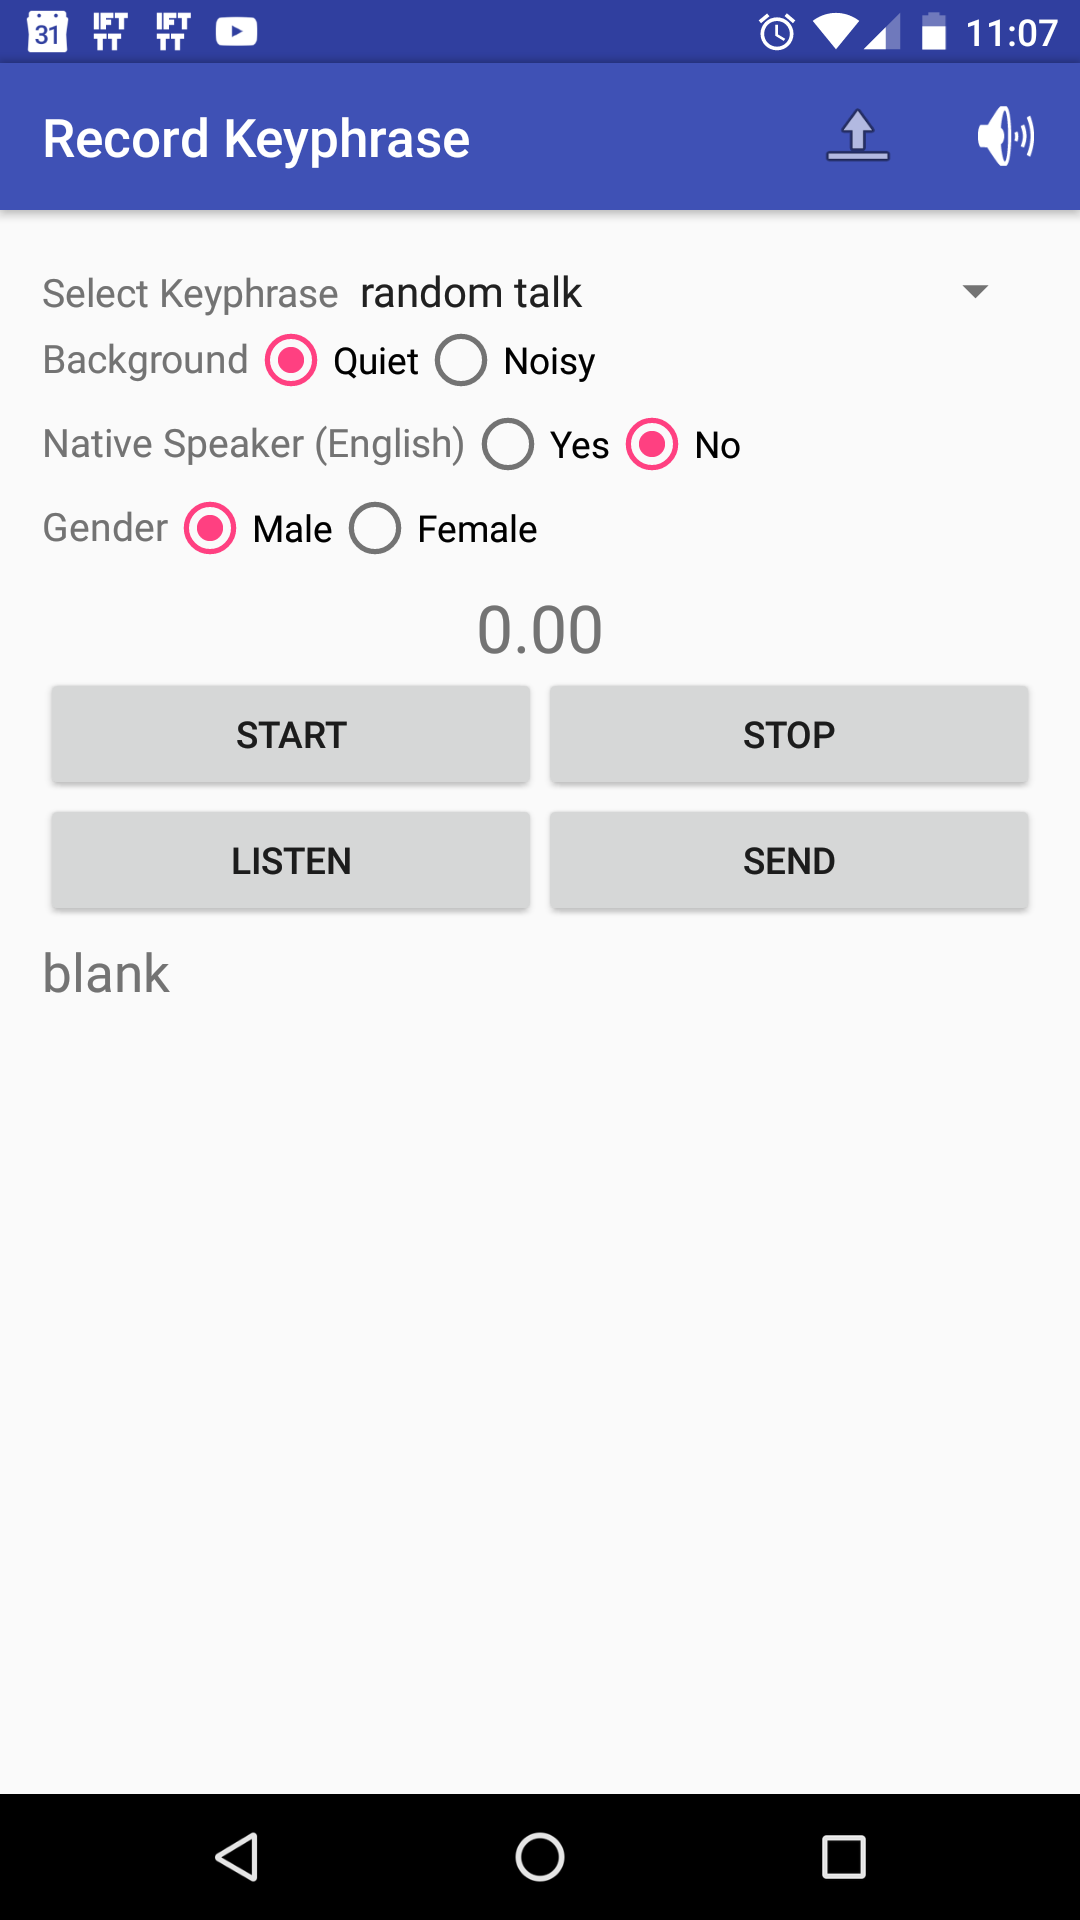
\includegraphics[width=0.25\textwidth]{sound/app_submit.png}
\caption{\texttt{dbHound Keyphrase} Android app screenshot for submitting training data}
\label{fig:dbhound_submit}
\end{figure}

\begin{figure}[!th]
\centering
\begin{subfigure}{0.5\textwidth}
\centering
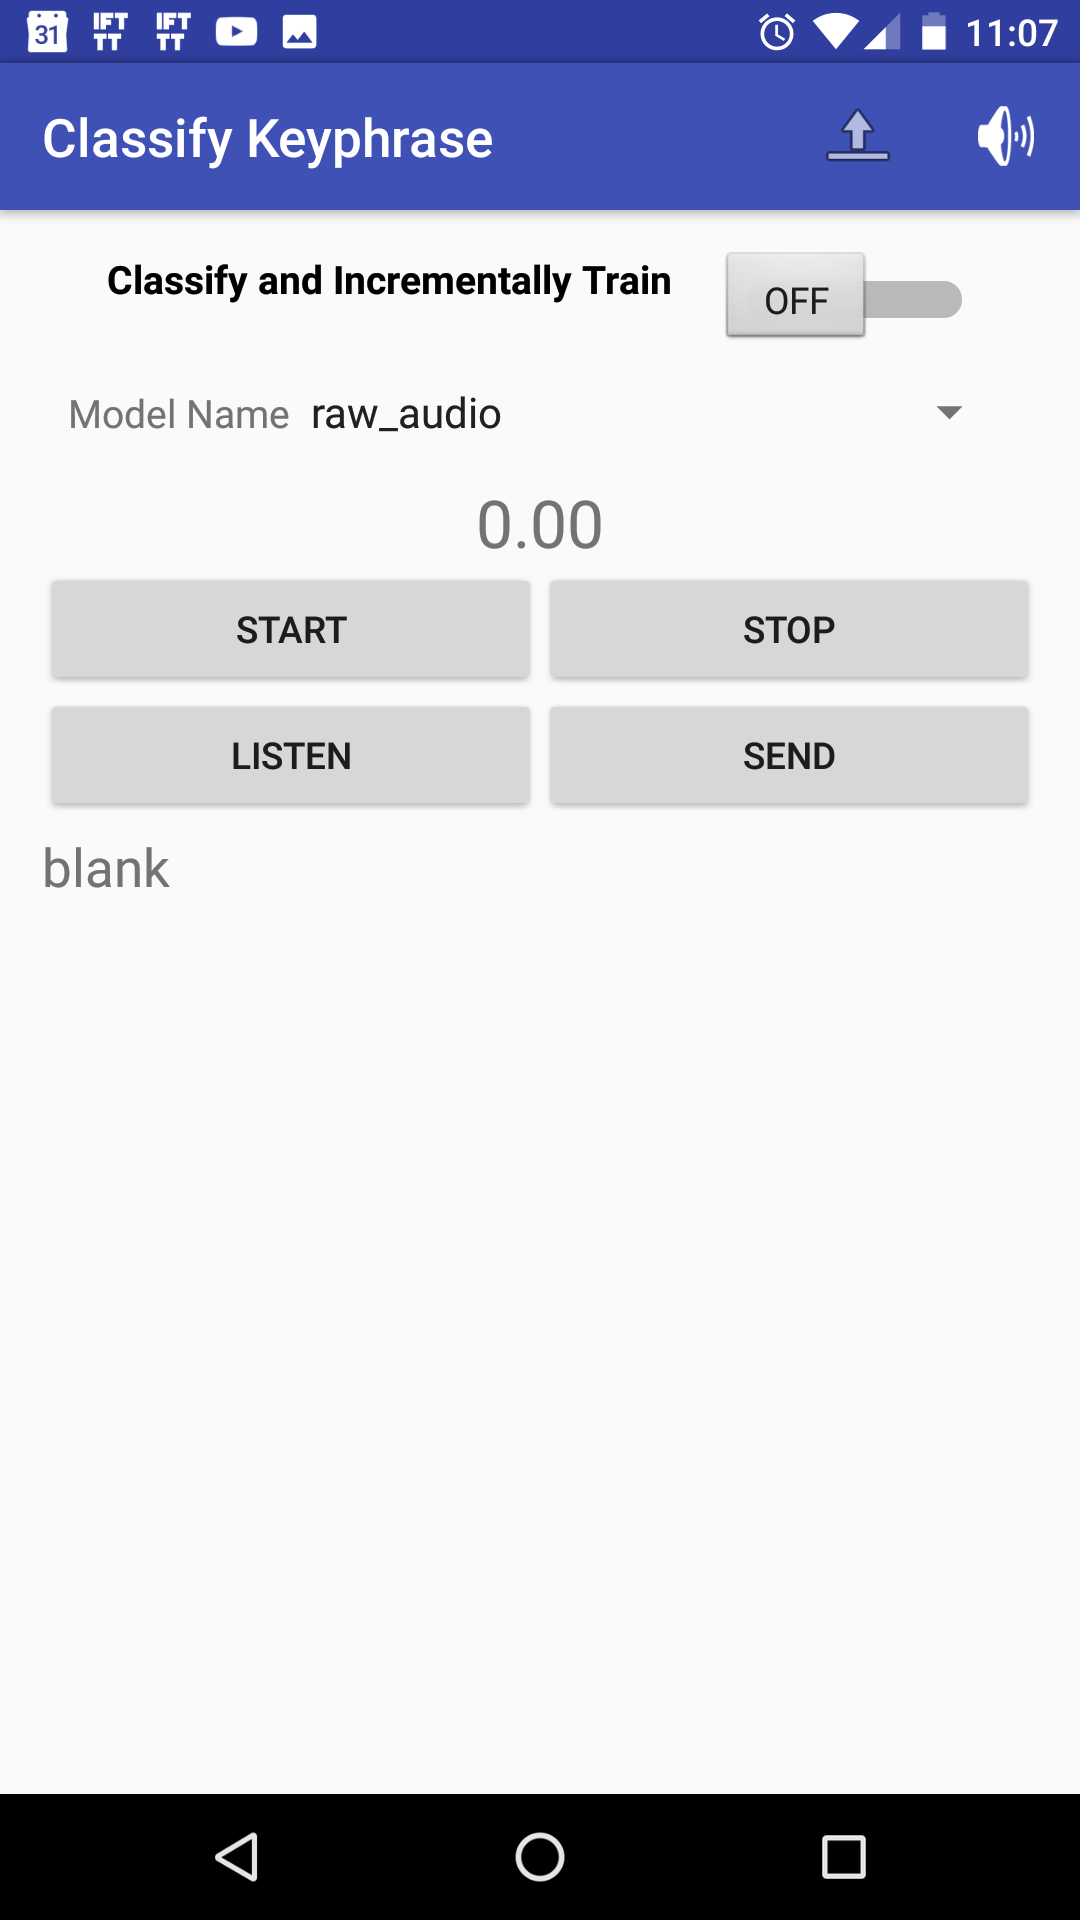
\includegraphics[width=0.5\textwidth]{sound/app_classify.png}
\caption{Only Classify}
\end{subfigure}%
\begin{subfigure}{0.5\textwidth}
\centering
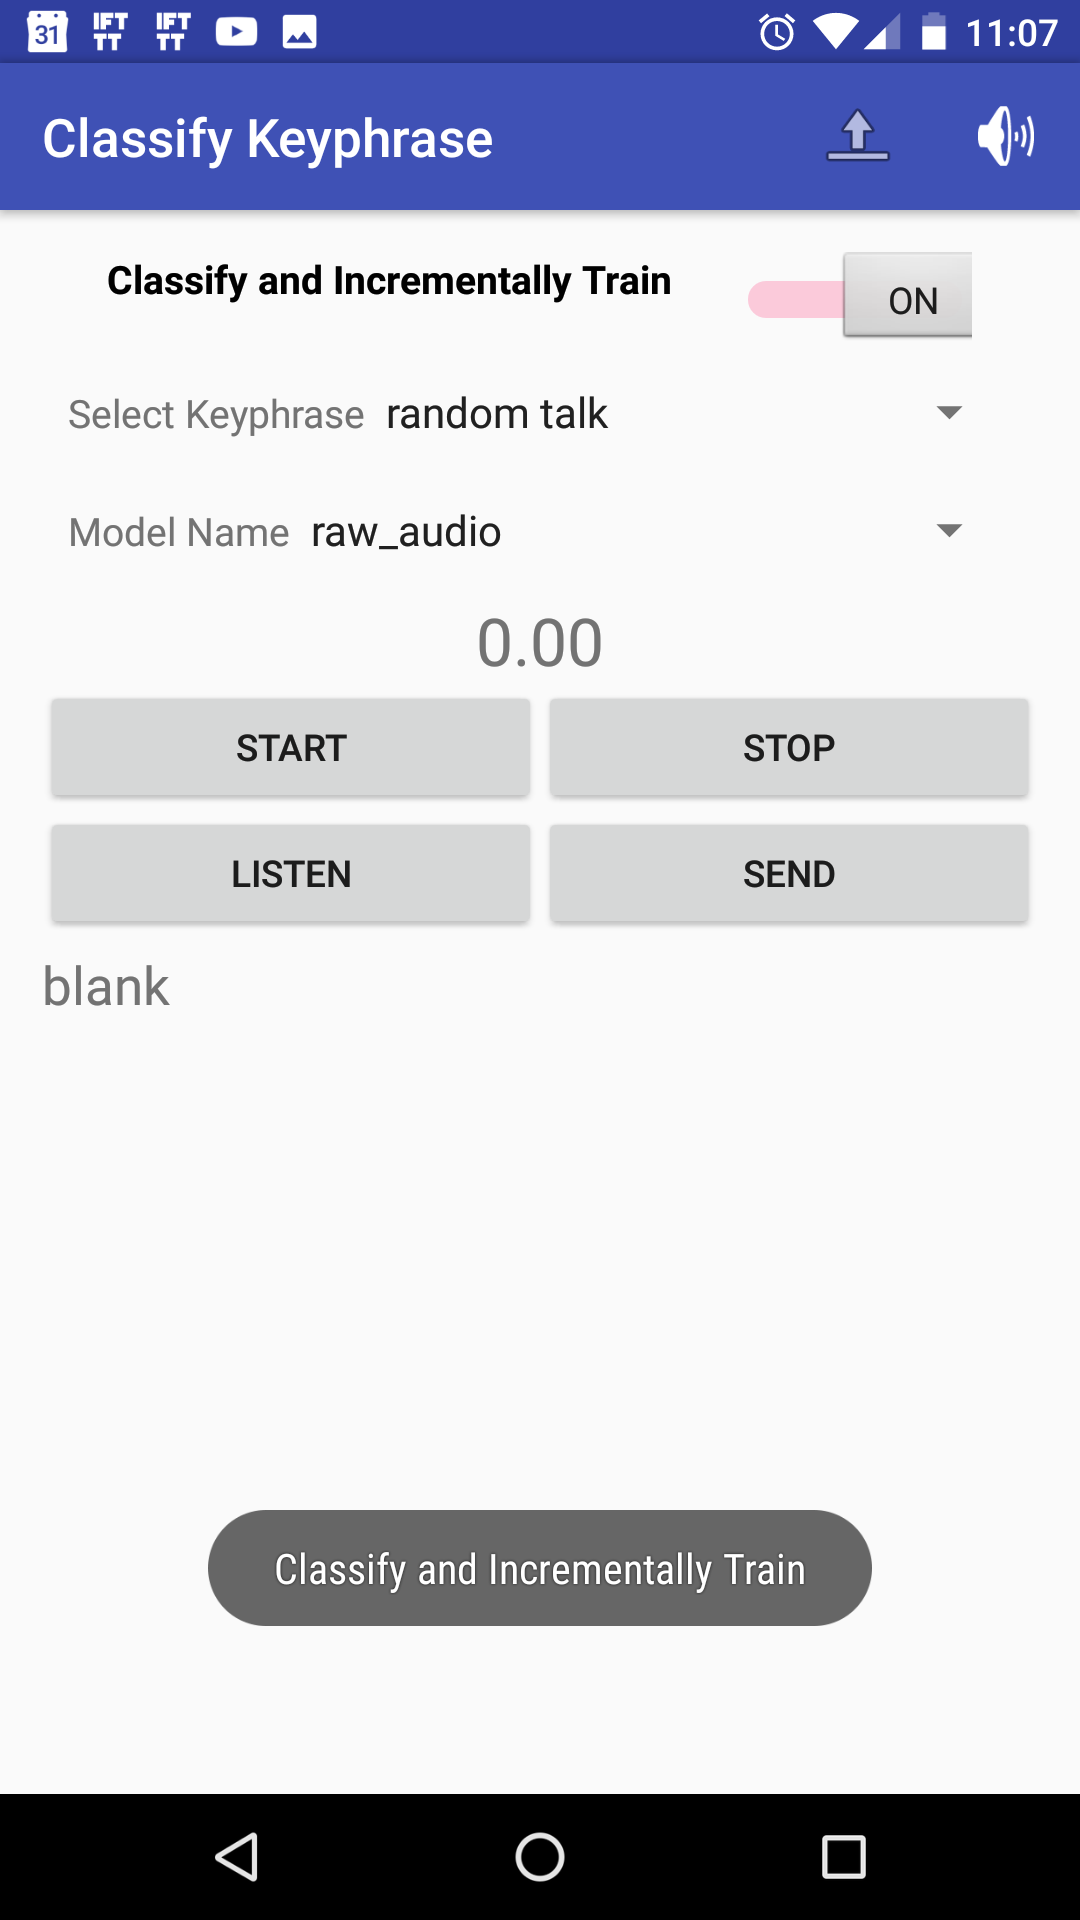
\includegraphics[width=0.5\textwidth]{sound/app_classify_and_train.png}
\caption{Classify and "Fine-Tune" Model}
\end{subfigure}%
\caption{\texttt{dbHound Keyphrase} Android app screenshot for testing the classification models}
\label{fig:dbhound_test}
\end{figure}

For preserving privacy, I propose a two-part solution:
\begin{itemize}
\item A computationally light transformation that removes conversational information from audio but preserves the ability to recognize a desired list of keywords.
\item A computationally light inference technique to spot the keywords from a stream of transformed audio data.
\end{itemize}





\section{Lightweight Audio Obfuscation}
\label{sec:obfuscation}

\TODO{small overview of both methods}

\TODO{describe data collected from mechanical turk in figure \ref{fig:mturk_survey}}. The first 4 bars correspond to decreasing decimated frequencies. \\ The last four bars correspond to decreasing bit depth of audio.

\afterpage{
    \begin{figure}[H]
    \centering
    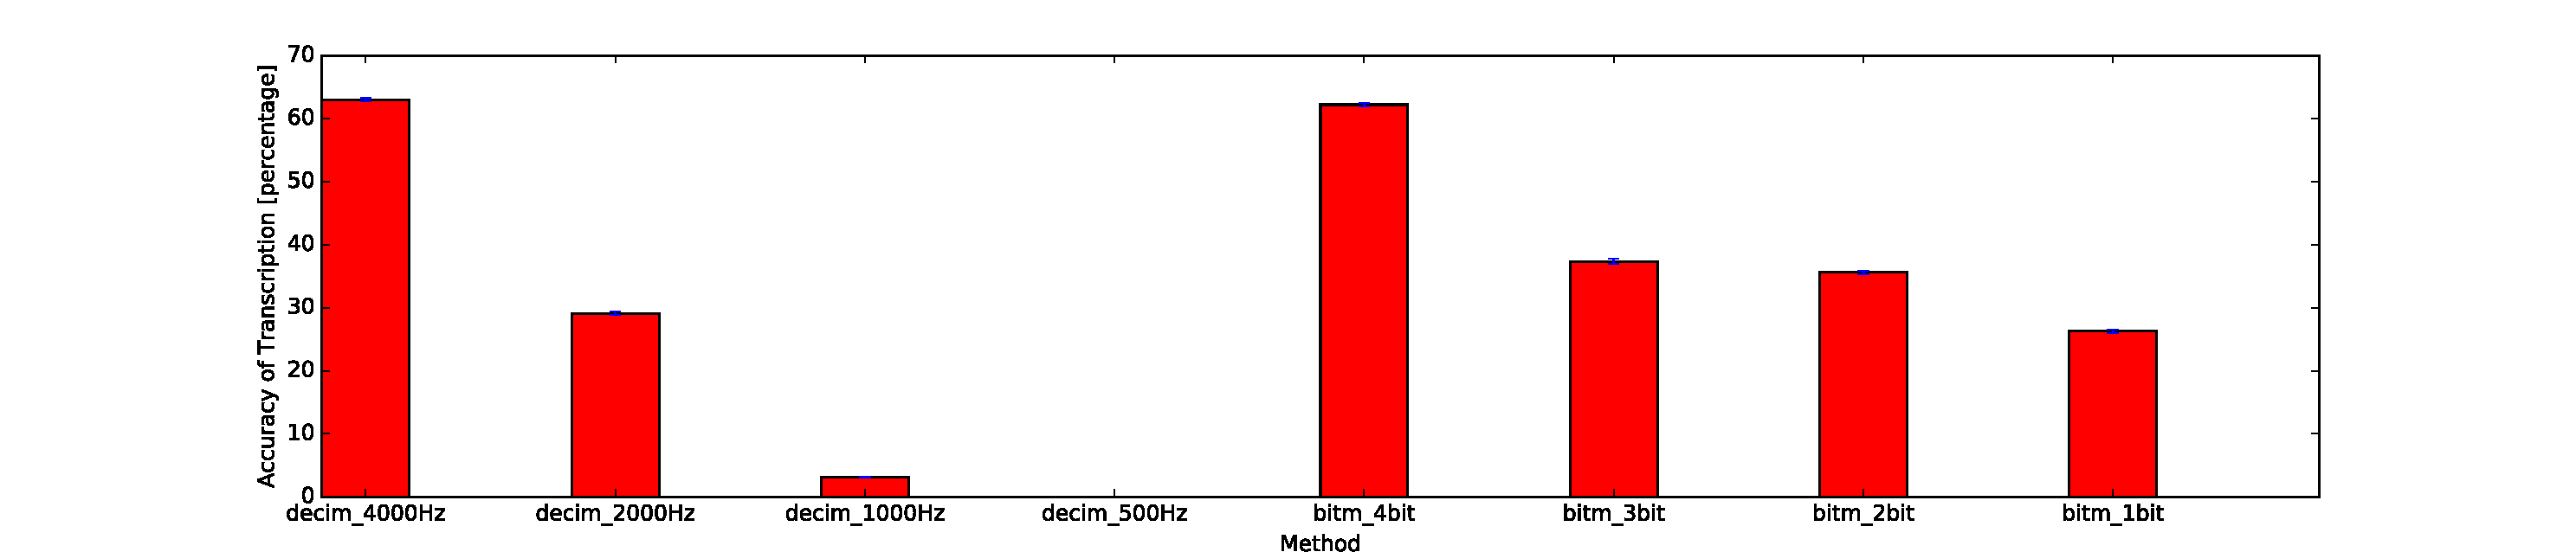
\includegraphics[width=\textwidth]{sound/mturk_survey.pdf}
    \caption{Accuracy of human transcription for different levels of decimation and quantization.}
    \label{fig:mturk_survey}
    \end{figure}
    \begin{table}[H]
    \begin{tabularx}{\textwidth}{l | l | l | l}
    \textbf{Key} & \textbf{Description} & \textbf{Key} & \textbf{Description} \\
    \hline
    decim\_4000 & Decimated to 4 kHZ & bitm\_4bit & 4-bit precision audio \\
    decim\_2000 & Decimated to 2 kHZ & bitm\_3bit & 3-bit precision audio \\
    decim\_1000 & Decimated to 1 kHZ & bitm\_2bit & 2-bit precision audio \\
    decim\_500 & Decimated to 500 HZ & bitm\_1bit & 1-bit precision audio \\
    \end{tabularx}
    \caption{Key for X-axis in Figure \ref{fig:mturk_survey}: \nameref{fig:mturk_survey}}
    \label{tab:key_mturk_survey}
    \end{table}
}

\subsection{Decimation: Removing time fidelity}

If the audio stream is recorded at 16kHz, we decimate the audio stream to a much lower sampling frequency.
 With this operation, the intelligibility of speech rapidly decreases with the amount of decimation.
 However, this also significantly decreases keyword spotting performance.

\TODO{ some raw data vs subsampled data? and the FFT for both to visualize information loss?}

\TODO{figure showing the performance decline of CMUSphinx, Google Speech Recog. with subsampled audio data}

\TODO{discuss the entropy and information content after this operation with respect to the raw audio}

\TODO{use differential privacy to discuss how adding controlled noise to this can prevent an attacker from understanding sensitive information.}


\subsection{Bit Depth: Removing amplitude fidelity}

If the audio stream is recorded at a 16-bit depth, we quantize the audio stream to a much lower bit depth to reduce the information content.
 Surprisingly, we find that, even at the lowest possible 1-bit depth, the speech content can be easily understood by humans (Figure \ref{fig:mturk_survey}).

\TODO{discuss: the loss of information with quantization? not so much}

\TODO{discuss the entropy and information content after this operation with respect to the raw audio}

\TODO{use differential privacy to discuss how adding controlled noise to this can prevent an attacker from understanding sensitive information.}

\subsection{Obfuscating audio using hamming weights}

If we consider each audio sample as one "sample bit", then we can compute the hamming weight of $n$ sample bits.
 This is done by concatenating the sample bit strings and counting the total number of "1"s in the $n$-sample bit string.

\TODO{discuss the entropy and information content after this operation with respect to the raw audio}

\TODO{use differential privacy to discuss how adding controlled noise to this can prevent an attacker from understanding sensitive information.}

\TODO{repeat the two analyses above applying the same hamming weight technique to both decimated audio and low bit-depth audio}

\subsection{Adding keywords to the dictionary}

\TODO{how would adding more keywords affect the privacy vs utility?}

\TODO{can we say if we add keywords with certain characteristics the algorithm will still be fine?}



\section{Keyphrase Recognition from Obfuscated Audio}
\label{sec:recognition_models}

I propose a deep neural network architecture (Figure \ref{fig:convnet_architecture}) to achieve this keyphrase recognition task in real time.
 Research work from Google in the past \cite{smallfootprintkeywordspotting} \cite{cnnkeywordspotting} \cite{chen2015locallyconnected} \cite{chen2014low} have shown that deep convolutional neural networks are suitable for online keyphrase recognition in mobile devices.
 The focus of my work is to survey the trade-off between privacy and keyphrase recognition performance for different audio obfuscation techniques.
 Based on the work from Google, I add the remark that efficient implementations of such architectures have been realized for mobile devices and it will be possible to translate the architecture I propose in a similar fashion, to mobile devices to realize the recommendations in Section \ref{sec:proposed_changes_to_mobile}.

The different layers of the deep convolutional neural network are described in detail below.

\subsection{Input Layer}

This contains all the samples from the obfuscated audio for a 2.048 second interval, with the audio being sampled at 16 kHz with 16-bit resolution.
 The interval of 2.048 seconds was chosen so that the corresponding number of raw audio samples is a power of 2 (32768 raw audio samples).
 This choice is purely one of convenience for signal processing.


Based on the obfuscation technique applied, the total number of samples provided in the input layer may be different.
 Some examples for this are shown in Table \ref{tab:input_layer_samples}.
 However, all of these variants still correspond to a time interval of 2.048 seconds, assisting in the consistency of the deep convolutional neural network across different obfuscation techniques.


For the sake of clarity when working with convolutional layers, the shape of the input layer can be re-written in the following manner.

\begin{gather}
\text{Shape Template} = (\text{height} \times \text{width} \times \text{channels}) \\
\text{Shape of Input Layer} = (N \times 1 \times 1)
\end{gather}

\begin{table}[!th]
\centering
\begin{tabularx}{\textwidth}{l | l}
\textbf{Obfuscation Technique} & \textbf{Input Layer Size} \\
\hline
No Obfuscation (Raw Audio) & 32768 \\
Decimation to 4 kHz & 8192 \\
Decimation to 1 kHz with 8-Hamming Reduction & 1024 \\
Decimation to 1 kHz & 2048 \\
Decimation to 1 kHz with 2-Hamming Reduction & 1024 \\
Bit Depth to 1 bit & 32768 \\
Bit Depth to 1 bit with 8-Hamming Reduction & 4096 \\
\end{tabularx}
\caption{Example list of size of input layer in the Deep Convolutional Neural Network for various obfuscation techniques}
\label{tab:input_layer_samples}
\end{table}

\subsection{Convolutional Layers}

In this case, I propose using 3 cascaded convolutional layers (interspersed with 3 max-pooling layers) to learn audio features for the classification task.
 Since the "width" (from the shape template above) is always 1, these layers can also be likened to a 1-D convolutional operation.
 Each convolutional layer is completely defined by the parameters described below. \footnote{Chris Olah's explanation in \cite{cnn_modular} is a great resource to understand the structure of ConvNets.}

\begin{itemize}
\item \textbf{Filter Size $(S)$:} The size of the convolutional filter defines the number of samples to work with to generate a feature.
 This also decides the size of the weight matrix for a single convolutional filter.
 For example, if only one filter of size $(20 \times 1 \times 1)$ is present, the filter works with 20 audio samples and 1 channel
 In other words, 20 weight variables are learnt per filter.
 The filter width is always 1, since this is a 1-D signal, and typically the filter works with all the channels of the input.
 Consequently, the filter size $S$ can be defined by a single number, 20, in this case.

\item \textbf{Filter Strides $(P)$:} The term "convolution" applies here because of the striding operation.
 Once the size of the convolutional filter is decided, the filter walks over sub-sections of the input space to compute a feature for different parts of the input.
 This can be likened to computing the Fourier Transform of different portions of a signal to understand localized frequency distributions --- the convolutional filter learns to find the best localized features.
 Clearly, given the high sample frequency of audio signals, striding the filter sample by sample would result in excessive computational time.
 Moreover, striding sample by sample is not likely to provide accuracy benefits either --- owing to the high sample frequency, the information (or phoneme) content is dispersed.
 The Filter Strides $P$ is the number of samples the filter "walks" over before computing the next feature.


Decreasing this parameter results in the filter striding in shorter steps (more instances of the same filter), increasing computation time while learning and evaluating.
 The size of the model (in terms of memory), however, remains unchanged.

\item \textbf{Number of Filters $(K)$:} This is used to set the number of filters (different features) to learn from the input.
 This can be likened to computing different types of transforms (e.g. fourier, haar, daubechies, cepstral etc.) over the same sub-sections of the input data.
 The intuition behind this is that different filters are likely to capture the essential features of the signal when used together.

\item \textbf{Activation Function:} This is the activation function used to generate the output at each node.
 Typical choices are ReLU, Sigmoid, tanh etc.

\end{itemize}

The size of the output of the 1-D convolutional filter is described below.
 The structure of my proposed deep convolutional neural network is described in \ref{tab:conv_layer_list}.

\begin{gather}
\text{Shape Template} = (\text{height} \times \text{width} \times \text{channels}) \\
\text{Shape of Input Layer} = (N \times 1 \times C) \\
\text{Shape of Output Layer} = \left(\frac{N-S+1}{P}, 1, K \right)
\end{gather}

The max-pooling layers are equivalent to a subsampling operation.
 They are introduced to maintain local translational invariance in the model.
 Consequently, a max-pooling operation of 4 decreases the number of input samples by a factor of $\left(\frac{1}{4}\right)$ in the output.
 The number 4 here is referred to as the "kernel size" of the max-pooling layer.
 It is standard practice for a max-pooling layer to follow a convolutional layer.
 \footnote{The Convolutional Layer together with its Max-Pooling Layer will be referred to as Conv-Max layer in the rest of this thesis.}
 All the max-pooling layers used in the architecture in Figure \ref{fig:convnet_architecture} have kernel size 2.

\begin{table}[!th]
\centering
\def\arraystretch{2}\tabcolsep=10pt

\begin{subtable}{\textwidth}
\centering
\begin{tabular}{l | l | l}
\textbf{Parameter} & \textbf{Convolutional Layer: 1} & \textbf{Convolutional Layer: 2} \\
\hline
Filter Size & $S = \frac{N}{128} \sim 16 ms$ & $S = 2 \sim 32 ms$ \\
Filter Strides & $P = \frac{S}{2} = \frac{N}{256}$ & $P = \frac{S}{2} = 1$ \\
Number of Filters & 1024 & 512 \\
Activation Function & ReLU & ReLU \\
Regularization & $L_2$ & $L_2$ \\
\end{tabular}
\end{subtable}

\vspace{3cm}

\begin{subtable}{\textwidth}
\centering
\begin{tabular}{l | l}
\textbf{Parameter} & \textbf{Convolutional Layer: 3} \\
\hline
Filter Size & $S = 8 \sim 256 ms$ \\
Filter Strides & $P = \frac{S}{2} = 4$ \\
Number of Filters & 128 \\
Activation Function & ReLU \\
Regularization & $L_2$ \\
\end{tabular}
\end{subtable}

\caption{Description of filter size for the Deep Convolutional Neural Network Architecture in Figure \ref{fig:convnet_architecture}. The input layer has $N$ samples.}
\label{tab:conv_layer_list}
\end{table}

\subsection{Densely Connected Layers}

The cascaded convolutional layers are used to learn the "best" features for the classification task at hand.
 The densely connected layers are intended to learn the actual classification task from the "best" features.
 If the output of the cascaded convolutional layers are considered as "features", then the rest of the network is a two-layer perceptron.
 In other words, the rest of the network can be treated as a neural network with one hidden layer and one output layer.

The hidden layer has ReLU activation with dropout regularization (the dropout probability is chosen as 0.8).
 The output layer has a softmax activation function to compute class probabilities.


When the neural network is fine-tuned online by the dbHound system, only the weights for the densely connected layers (two-layer perceptron) are updated.
 The reason only the two-layer perceptron is fine-tuned is to prevent overfitting on new data --- using this approach, the feature computation is "frozen" and the classification boundary is \textbf{slightly} nudged to accommodate new examples.
 This "incremental" learning is also done with a very small learning rate with the idea that the classifier is already well learnt and only needs to be slightly adapted to deal with new data.

\begin{figure}[!t]
\centering
\tikzset{%
    cascaded/.style={%
        general shadow={%
            shadow scale=1,
            shadow xshift=-1ex,
            shadow yshift=1ex,
            draw,
            thick,
            fill=white
        },
        general shadow={%
            shadow scale=1,
            shadow xshift=-.5ex,
            shadow yshift=.5ex,
            draw,
            thick,
            fill=white
        },
        fill=white,
        draw,
        thick,
        minimum width=1.5cm,
        minimum height=2cm
    }
}

\tikzstyle{vecArrowShort}=[thick,
                      shorten >= 5.5pt,
                      postaction={draw,line width=2pt, black, shorten >= 4.5pt}
]
\tikzstyle{vecArrow}=[thick,
                      postaction={draw,line width=2pt, black}
]

\tikzstyle{maxpool} = [rectangle, draw, fill=yellow!20, text centered, rounded corners]
\tikzstyle{conv} = [rectangle, draw, fill=blue!20, text centered, rounded corners, minimum height=4em, minimum width=20em]
\tikzstyle{shortline} = [draw, -latex', fill=black, vecArrowShort]
\tikzstyle{line} = [draw, -latex', fill=black, vecArrow]
\tikzstyle{dense} = [draw, ellipse,fill=red!20, minimum height=2em]
\tikzstyle{input} = [rectangle, draw, fill=green!20, text centered, sharp corners, minimum height=2em, minimum width=15em, align=center]
\tikzstyle{output} = [rectangle, draw, fill=green!20, text centered, sharp corners, minimum height=2em, minimum width=5em, align=center]

\begin{tikzpicture}[node distance = 2cm, auto]

% nodes
\node [input] (input) { $N \text{Audio Samples}$ };
\node [cascaded, conv, below of=input] (conv1) { $\text{1-D Convolutional Layer: 1}$ };
\node [maxpool, below of=conv1] (maxpool1) { Max-Pool Layer: 1 };
\node [cascaded, conv, below of=maxpool1] (conv2) { $\text{1-D Convolutional Layer: 2}$ };
\node [maxpool, below of=conv2] (maxpool2) { Max-Pool Layer: 2 };
\node [cascaded, conv, below of=maxpool2] (conv3) { $\text{1-D Convolutional Layer: 3}$ };
\node [maxpool, below of=conv3] (maxpool3) { Max-Pool Layer: 3 };
\node [dense, below of=maxpool3] (dense1) { $\text{Fully Connected Layer: 1}$ };
\node [dense, below of=dense1] (dense2) { $\text{Fully Connected Layer: 2}$ };
\node [output, below of=dense2] (output) { $(2 \times 1)$ softmax output };

%arrows
\path [shortline] (input) -- (conv1);
\path [line] (conv1) -- (maxpool1);
\path [shortline] (maxpool1) -- (conv2);
\path [line] (conv2) -- (maxpool2);
\path [shortline] (maxpool2) -- (conv3);
\path [line] (conv3) -- (maxpool3);
\path [line] (maxpool3) -- (dense1);
\path [line] (dense1) -- (dense2);
\path [line] (dense2) -- (output);

\end{tikzpicture}
\caption{Architecture of the Deep Convolutional Neural Network for Keyphrase Recognition}
\label{fig:convnet_architecture}
\end{figure}





\section{Evaluating Keyphrase Recognition Performance}
\label{sec:recognition_evaluation}

In this section, I present performance results for the ensemble of classification models learnt from keyphrase data.
 The model is organized as follows:

\begin{itemize}
\item An individiual classification model is learnt for every keyphrase apart from "random talk".
 The objective of the classification is to distinguish between the true keyphrase and "random talk".
\item For a test audio clip, all 8 classification models are used to get class probabilities for the associated keyphrase.
 The keyphrase with the maximum class probability is chosen and compared to a confidence threshold.
 If the class probability is greater or equal to than the confidence threshold, the classification output is the true keyphrase.
 If the class probability is lower than the confidence threshold, the classification output is "random talk".
\end{itemize}


Summarized in \cref{tab:probs_raw_audio,tab:probs_raw_audio_hamming_1,tab:probs_raw_audio_hamming_4,tab:probs_raw_audio_hamming_16,tab:probs_samplerate_2000,tab:probs_samplerate_1000,tab:probs_samplerate_2000_hamming_1,tab:probs_samplerate_1000_hamming_1,tab:probs_samplerate_2000_hamming_4,tab:probs_samplerate_1000_hamming_4,tab:probs_samplerate_2000_hamming_16,tab:probs_precision_1_hamming_1,tab:probs_precision_1_hamming_4,tab:probs_precision_1_hamming_16}
 are the mean class probabilities for different keyphrase audio examples using different keyphrase models.
 Each table corresponds to a different obfuscation technique, as noted in the caption.
 Each table corresponds to a different obfuscation technique.
 Each row corresponds to a classification model for a single keyphrase.
 Each column corresponds to audio examples for a single keyphrase, or audio examples for "random talk".
 The class probabilities in the table indicate the level to which the model has learnt the training set.


Examples for "random talk" are an assortment of choices from three sources:
\begin{itemize}
\item TED-LIUM Speech Corpus
\item Babble Noise Examples (Cafeteria noise, Public Transit Vehicle Noise)
\item "random talk" examples from the \texttt{dbHound Keyphrase}\footnote{The \texttt{dbHound Keyphrase} android application can be found on the Google Play Store at \url{https://play.google.com/store/apps/details?id=edu.wisc.cs.dbhound}.} android application
\end{itemize}

Figures \ref{fig:roc_raw_audio} \ref{fig:roc_samplerate} \ref{fig:roc_precision_bits} show the Receiver Operating Curves (ROC) for different obfuscation techniques.
 The Receiver Operating Curve shows the variation of the false positive ratio and true positive ratio when the confidence threshold for classification is varied.
 These curves help understand how well the model is likely to perform in real life.


\begin{table}[!th]
\begin{tabular}{cccccccccc}%
\hline%
None&\rotate{random talk}{70}&\rotate{okay google}{70}&\rotate{hey siri}{70}&\rotate{hey cortana}{70}&\rotate{nine one one}{70}&\rotate{call mom}{70}&\rotate{take a picture}{70}&\rotate{play a song}{70}&\rotate{make a note}{70}\\%
\hline%
okay google&0.01&\textbf{0.83}&0.01&0.01&0.0&0.0&0.01&0.0&0.01\\%
hey siri&0.01&0.05&\textbf{0.64}&0.01&0.0&0.0&0.09&0.03&0.02\\%
hey cortana&0.01&0.03&0.03&\textbf{0.66}&0.04&0.02&0.02&0.02&0.02\\%
nine one one&0.0&0.0&0.0&0.0&\textbf{0.83}&0.03&0.0&0.01&0.01\\%
call mom&0.01&0.0&0.01&0.06&0.03&\textbf{0.94}&0.0&0.05&0.0\\%
take a picture&0.01&0.02&0.03&0.01&0.0&0.0&\textbf{0.77}&0.0&0.01\\%
play a song&0.02&0.01&0.03&0.02&0.01&0.04&0.01&\textbf{0.71}&0.03\\%
make a note&0.02&0.03&0.02&0.02&0.01&0.03&0.03&0.01&\textbf{0.67}\\%
\hline%
\end{tabular}
\caption{Mean Class Probabilities from 350 audio examples. Each row corresponds to a different keyphrase classification model. Each column corresponds to a different keyphrase audio example. \emph{Obfuscation technique: no obfuscation}}
\label{tab:probs_raw_audio}
\end{table}



\begin{table}[!th]
\begin{tabular}{cccccccccc}%
\hline%
None&\rotate{random talk}{70}&\rotate{okay google}{70}&\rotate{hey siri}{70}&\rotate{hey cortana}{70}&\rotate{nine one one}{70}&\rotate{call mom}{70}&\rotate{take a picture}{70}&\rotate{play a song}{70}&\rotate{make a note}{70}\\%
\hline%
okay google&0.07&\textbf{0.52}&0.06&0.12&0.09&0.1&0.08&0.08&0.1\\%
hey siri&0.1&0.14&\textbf{0.53}&0.14&0.12&0.09&0.14&0.13&0.11\\%
hey cortana&0.06&0.09&0.08&\textbf{0.58}&0.07&0.08&0.11&0.08&0.11\\%
nine one one&0.02&0.04&0.04&0.03&\textbf{0.77}&0.12&0.02&0.08&0.05\\%
call mom&0.01&0.01&0.03&0.04&0.05&\textbf{0.83}&0.02&0.1&0.06\\%
take a picture&0.01&0.05&0.03&0.07&0.06&0.03&\textbf{0.38}&0.09&0.05\\%
play a song&0.0&0.01&0.01&0.03&0.03&0.05&0.01&\textbf{0.39}&0.02\\%
make a note&0.04&0.06&0.08&0.06&0.1&0.08&0.05&0.08&\textbf{0.44}\\%
\hline%
\end{tabular}
\caption{Mean Class Probabilities from 350 audio examples. Each row corresponds to a different keyphrase classification model. Each column corresponds to a different keyphrase audio example. \emph{Obfuscation technique: hamming reduction on every 1 sample}}
\label{tab:probs_raw_audio_hamming_1}
\end{table}





\begin{table}[!th]
\begin{tabular}{cccccccccc}%
\hline%
None&\rotate{random talk}{70}&\rotate{okay google}{70}&\rotate{hey siri}{70}&\rotate{hey cortana}{70}&\rotate{nine one one}{70}&\rotate{call mom}{70}&\rotate{take a picture}{70}&\rotate{play a song}{70}&\rotate{make a note}{70}\\%
\hline%
okay google&0.04&\textbf{0.79}&0.06&0.12&0.03&0.03&0.07&0.05&0.05\\%
hey siri&0.06&0.07&\textbf{0.45}&0.08&0.04&0.05&0.07&0.04&0.05\\%
hey cortana&0.01&0.07&0.04&\textbf{0.57}&0.01&0.02&0.08&0.03&0.05\\%
nine one one&0.02&0.03&0.04&0.03&\textbf{0.64}&0.15&0.02&0.07&0.03\\%
call mom&0.0&0.0&0.02&0.02&0.05&\textbf{0.71}&0.01&0.05&0.05\\%
take a picture&0.03&0.05&0.02&0.05&0.01&0.01&\textbf{0.63}&0.02&0.02\\%
play a song&0.04&0.05&0.07&0.06&0.13&0.1&0.06&\textbf{0.32}&0.09\\%
make a note&0.0&0.01&0.01&0.02&0.02&0.03&0.02&0.04&\textbf{0.52}\\%
\hline%
\end{tabular}
\caption{Mean Class Probabilities from 350 audio examples. Each row corresponds to a different keyphrase classification model. Each column corresponds to a different keyphrase audio example. \emph{Obfuscation technique: hamming reduction on every 4 samples}}
\label{tab:probs_raw_audio_hamming_4}
\end{table}





\begin{table}[!th]
\begin{tabular}{cccccccccc}%
\hline%
None&\rotate{random talk}{70}&\rotate{okay google}{70}&\rotate{hey siri}{70}&\rotate{hey cortana}{70}&\rotate{nine one one}{70}&\rotate{call mom}{70}&\rotate{take a picture}{70}&\rotate{play a song}{70}&\rotate{make a note}{70}\\%
\hline%
okay google&0.03&\textbf{0.85}&0.0&0.09&0.0&0.0&0.01&0.0&0.0\\%
hey siri&0.0&0.0&\textbf{0.99}&0.0&0.0&0.0&0.0&0.0&0.0\\%
hey cortana&0.01&0.02&0.02&\textbf{0.91}&0.01&0.01&0.0&0.02&0.03\\%
nine one one&0.01&0.0&0.0&0.01&\textbf{0.98}&0.0&0.0&0.01&0.0\\%
call mom&0.0&0.0&0.01&0.0&0.0&\textbf{0.81}&0.0&0.01&0.0\\%
take a picture&0.0&0.0&0.0&0.0&0.0&0.0&\textbf{0.7}&0.0&0.0\\%
play a song&0.0&0.0&0.0&0.01&0.01&0.01&0.0&\textbf{0.68}&0.0\\%
make a note&0.02&0.0&0.0&0.0&0.0&0.0&0.0&0.0&\textbf{0.87}\\%
\hline%
\end{tabular}
\caption{Mean Class Probabilities from 350 audio examples. Each row corresponds to a different keyphrase classification model. Each column corresponds to a different keyphrase audio example. \emph{Obfuscation technique: hamming reduction on every 16 samples}}
\label{tab:probs_raw_audio_hamming_16}
\end{table}



\clearpage


\begin{table}[!th]
\begin{tabular}{cccccccccc}%
\hline%
None&\rotate{random talk}{70}&\rotate{okay google}{70}&\rotate{hey siri}{70}&\rotate{hey cortana}{70}&\rotate{nine one one}{70}&\rotate{call mom}{70}&\rotate{take a picture}{70}&\rotate{play a song}{70}&\rotate{make a note}{70}\\%
\hline%
okay google&0.03&\textbf{0.73}&0.03&0.02&0.01&0.0&0.05&0.01&0.02\\%
hey siri&0.01&0.03&\textbf{0.51}&0.03&0.01&0.02&0.05&0.02&0.03\\%
hey cortana&0.02&0.05&0.03&\textbf{0.74}&0.02&0.02&0.05&0.03&0.01\\%
nine one one&0.04&0.03&0.02&0.07&\textbf{0.87}&0.04&0.03&0.03&0.02\\%
call mom&0.0&0.0&0.02&0.02&0.04&\textbf{0.92}&0.0&0.08&0.02\\%
take a picture&0.02&0.02&0.04&0.01&0.0&0.0&\textbf{0.49}&0.01&0.01\\%
play a song&0.01&0.01&0.1&0.04&0.03&0.13&0.01&\textbf{0.81}&0.04\\%
make a note&0.04&0.06&0.03&0.03&0.04&0.03&0.02&0.04&\textbf{0.58}\\%
\hline%
\end{tabular}
\caption{Mean Class Probabilities from 350 audio examples. Each row corresponds to a different keyphrase classification model. Each column corresponds to a different keyphrase audio example. \emph{Obfuscation technique: samplerate reduced to 2000 Hz}}
\label{tab:probs_samplerate_2000}
\end{table}







\begin{table}[!th]
\begin{tabular}{cccccccccc}%
\hline%
None&\rotate{random talk}{70}&\rotate{okay google}{70}&\rotate{hey siri}{70}&\rotate{hey cortana}{70}&\rotate{nine one one}{70}&\rotate{call mom}{70}&\rotate{take a picture}{70}&\rotate{play a song}{70}&\rotate{make a note}{70}\\%
\hline%
okay google&0.01&\textbf{0.34}&0.01&0.03&0.01&0.01&0.02&0.01&0.03\\%
hey siri&0.06&0.06&\textbf{0.06}&0.06&0.06&0.06&0.06&0.06&0.06\\%
hey cortana&0.01&0.04&0.07&\textbf{0.68}&0.03&0.01&0.03&0.08&0.04\\%
nine one one&0.01&0.01&0.02&0.01&\textbf{0.64}&0.02&0.02&0.02&0.01\\%
call mom&0.01&0.02&0.02&0.06&0.04&\textbf{0.62}&0.01&0.03&0.02\\%
take a picture&0.05&0.05&0.05&0.05&0.05&0.05&\textbf{0.05}&0.05&0.05\\%
play a song&0.04&0.05&0.11&0.03&0.09&0.11&0.03&\textbf{0.66}&0.06\\%
make a note&0.02&0.04&0.03&0.08&0.03&0.02&0.06&0.06&\textbf{0.26}\\%
\hline%
\end{tabular}
\caption{Mean Class Probabilities from 350 audio examples. Each row corresponds to a different keyphrase classification model. Each column corresponds to a different keyphrase audio example. \emph{Obfuscation technique: samplerate reduced to 1000 Hz}}
\label{tab:probs_samplerate_1000}
\end{table}





\begin{table}[!th]
\begin{tabular}{cccccccccc}%
\hline%
None&\rotate{random talk}{70}&\rotate{okay google}{70}&\rotate{hey siri}{70}&\rotate{hey cortana}{70}&\rotate{nine one one}{70}&\rotate{call mom}{70}&\rotate{take a picture}{70}&\rotate{play a song}{70}&\rotate{make a note}{70}\\%
\hline%
okay google&0.03&\textbf{0.49}&0.05&0.06&0.03&0.02&0.04&0.02&0.02\\%
hey siri&0.07&0.07&\textbf{0.43}&0.1&0.1&0.1&0.09&0.1&0.07\\%
hey cortana&0.02&0.06&0.04&\textbf{0.44}&0.01&0.01&0.06&0.01&0.02\\%
nine one one&0.03&0.04&0.05&0.04&\textbf{0.72}&0.16&0.02&0.09&0.04\\%
call mom&0.01&0.0&0.02&0.02&0.03&\textbf{0.55}&0.02&0.04&0.06\\%
take a picture&0.06&0.05&0.04&0.06&0.01&0.01&\textbf{0.63}&0.03&0.02\\%
play a song&0.01&0.0&0.01&0.01&0.05&0.07&0.01&\textbf{0.43}&0.05\\%
make a note&0.01&0.03&0.04&0.05&0.04&0.07&0.04&0.04&\textbf{0.42}\\%
\hline%
\end{tabular}
\caption{Mean Class Probabilities from 350 audio examples. Each row corresponds to a different keyphrase classification model. Each column corresponds to a different keyphrase audio example. \emph{Obfuscation technique: samplerate reduced to 2000 Hz followed by hamming reduction on every 1 sample}}
\label{tab:probs_samplerate_2000_hamming_1}
\end{table}








\begin{table}[!th]
\begin{tabular}{cccccccccc}%
\hline%
None&\rotate{random talk}{70}&\rotate{okay google}{70}&\rotate{hey siri}{70}&\rotate{hey cortana}{70}&\rotate{nine one one}{70}&\rotate{call mom}{70}&\rotate{take a picture}{70}&\rotate{play a song}{70}&\rotate{make a note}{70}\\%
\hline%
okay google&0.05&\textbf{0.86}&0.03&0.09&0.03&0.05&0.03&0.04&0.03\\%
hey siri&0.03&0.01&\textbf{0.96}&0.03&0.03&0.02&0.04&0.01&0.06\\%
hey cortana&0.01&0.01&0.01&\textbf{0.51}&0.01&0.01&0.01&0.01&0.01\\%
nine one one&0.0&0.0&0.0&0.0&\textbf{1.0}&0.0&0.0&0.0&0.0\\%
call mom&0.01&0.0&0.01&0.0&0.0&\textbf{0.99}&0.0&0.01&0.0\\%
take a picture&0.01&0.05&0.01&0.03&0.01&0.02&\textbf{0.87}&0.01&0.03\\%
play a song&0.02&0.0&0.0&0.0&0.03&0.0&0.01&\textbf{0.9}&0.0\\%
make a note&0.0&0.0&0.0&0.0&0.0&0.0&0.0&0.0&\textbf{1.0}\\%
\hline%
\end{tabular}
\caption{Mean Class Probabilities from 350 audio examples. Each row corresponds to a different keyphrase classification model. Each column corresponds to a different keyphrase audio example. \emph{Obfuscation technique: samplerate reduced to 1000 Hz followed by hamming reduction on every 1 sample}}
\label{tab:probs_samplerate_1000_hamming_1}
\end{table}









\begin{table}[!th]
\begin{tabular}{cccccccccc}%
\hline%
None&\rotate{random talk}{70}&\rotate{okay google}{70}&\rotate{hey siri}{70}&\rotate{hey cortana}{70}&\rotate{nine one one}{70}&\rotate{call mom}{70}&\rotate{take a picture}{70}&\rotate{play a song}{70}&\rotate{make a note}{70}\\%
\hline%
okay google&0.01&\textbf{0.84}&0.01&0.01&0.02&0.01&0.01&0.02&0.01\\%
hey siri&0.0&0.0&\textbf{0.99}&0.0&0.0&0.0&0.0&0.0&0.0\\%
hey cortana&0.04&0.04&0.06&\textbf{0.78}&0.01&0.0&0.04&0.02&0.03\\%
nine one one&0.01&0.0&0.0&0.04&\textbf{0.91}&0.0&0.01&0.02&0.01\\%
call mom&0.0&0.0&0.0&0.0&0.0&\textbf{0.28}&0.0&0.0&0.0\\%
take a picture&0.0&0.0&0.0&0.0&0.0&0.0&\textbf{1.0}&0.0&0.0\\%
play a song&0.01&0.0&0.0&0.0&0.0&0.0&0.0&\textbf{0.98}&0.0\\%
make a note&0.02&0.0&0.01&0.0&0.01&0.03&0.01&0.03&\textbf{0.86}\\%
\hline%
\end{tabular}
\caption{Mean Class Probabilities from 350 audio examples. Each row corresponds to a different keyphrase classification model. Each column corresponds to a different keyphrase audio example. \emph{Obfuscation technique: samplerate reduced to 2000 Hz followed by hamming reduction on every 4 samples}}
\label{tab:probs_samplerate_2000_hamming_4}
\end{table}







\begin{table}[!th]
\begin{tabular}{cccccccccc}%
\hline%
None&\rotate{random talk}{70}&\rotate{okay google}{70}&\rotate{hey siri}{70}&\rotate{hey cortana}{70}&\rotate{nine one one}{70}&\rotate{call mom}{70}&\rotate{take a picture}{70}&\rotate{play a song}{70}&\rotate{make a note}{70}\\%
\hline%
okay google&0.0&\textbf{0.48}&0.0&0.01&0.0&0.0&0.0&0.01&0.0\\%
hey siri&0.03&0.03&\textbf{0.72}&0.02&0.03&0.02&0.08&0.01&0.02\\%
hey cortana&0.02&0.06&0.04&\textbf{0.77}&0.03&0.03&0.01&0.03&0.11\\%
nine one one&0.02&0.02&0.01&0.01&\textbf{0.82}&0.04&0.01&0.01&0.01\\%
call mom&0.01&0.02&0.02&0.01&0.03&\textbf{0.1}&0.02&0.03&0.01\\%
take a picture&0.03&0.02&0.01&0.01&0.01&0.03&\textbf{0.88}&0.01&0.01\\%
play a song&0.01&0.05&0.03&0.02&0.06&0.05&0.01&\textbf{0.92}&0.02\\%
make a note&0.01&0.04&0.04&0.02&0.01&0.01&0.0&0.01&\textbf{0.73}\\%
\hline%
\end{tabular}
\caption{Mean Class Probabilities from 350 audio examples. Each row corresponds to a different keyphrase classification model. Each column corresponds to a different keyphrase audio example. \emph{Obfuscation technique: samplerate reduced to 1000 Hz followed by hamming reduction every 4 samples}}
\label{tab:probs_samplerate_1000_hamming_4}
\end{table}








\begin{table}[!th]
\begin{tabular}{cccccccccc}%
\hline%
None&\rotate{random talk}{70}&\rotate{okay google}{70}&\rotate{hey siri}{70}&\rotate{hey cortana}{70}&\rotate{nine one one}{70}&\rotate{call mom}{70}&\rotate{take a picture}{70}&\rotate{play a song}{70}&\rotate{make a note}{70}\\%
\hline%
okay google&0.02&\textbf{0.72}&0.02&0.06&0.06&0.01&0.06&0.08&0.04\\%
hey siri&0.01&0.05&\textbf{0.11}&0.05&0.06&0.1&0.04&0.06&0.08\\%
hey cortana&0.02&0.02&0.01&\textbf{0.99}&0.01&0.0&0.01&0.02&0.01\\%
nine one one&0.04&0.05&0.07&0.07&\textbf{0.73}&0.12&0.05&0.09&0.08\\%
call mom&0.0&0.01&0.02&0.0&0.02&\textbf{0.85}&0.0&0.09&0.04\\%
take a picture&0.0&0.0&0.0&0.0&0.0&0.0&\textbf{1.0}&0.0&0.0\\%
play a song&0.01&0.0&0.0&0.0&0.0&0.0&0.0&\textbf{0.98}&0.0\\%
make a note&0.01&0.0&0.0&0.0&0.0&0.0&0.0&0.0&\textbf{1.0}\\%
\hline%
\end{tabular}
\caption{Mean Class Probabilities from 350 audio examples. Each row corresponds to a different keyphrase classification model. Each column corresponds to a different keyphrase audio example. \emph{Obfuscation technique: samplerate reduced to 2000 Hz followed by hamming reduction on every 16 samples}}
\label{tab:probs_samplerate_2000_hamming_16}
\end{table}




\begin{table}[!th]
\begin{tabular}{cccccccccc}%
\hline%
None&\rotate{random talk}{70}&\rotate{okay google}{70}&\rotate{hey siri}{70}&\rotate{hey cortana}{70}&\rotate{nine one one}{70}&\rotate{call mom}{70}&\rotate{take a picture}{70}&\rotate{play a song}{70}&\rotate{make a note}{70}\\%
\hline%
okay google&0.0&\textbf{1.0}&0.0&0.0&0.0&0.0&0.0&0.0&0.0\\%
hey siri&0.0&0.0&\textbf{0.76}&0.0&0.0&0.0&0.0&0.0&0.0\\%
hey cortana&0.01&0.0&0.0&\textbf{0.99}&0.0&0.0&0.0&0.0&0.01\\%
nine one one&0.0&0.0&0.0&0.0&\textbf{1.0}&0.0&0.0&0.0&0.0\\%
call mom&0.0&0.0&0.0&0.0&0.0&\textbf{1.0}&0.0&0.0&0.0\\%
take a picture&0.02&0.0&0.0&0.0&0.0&0.0&\textbf{1.0}&0.0&0.0\\%
play a song&0.0&0.0&0.0&0.0&0.0&0.0&0.0&\textbf{1.0}&0.0\\%
make a note&0.01&0.02&0.0&0.0&0.0&0.05&0.0&0.03&\textbf{0.95}\\%
\hline%
\end{tabular}
\caption{Mean Class Probabilities from 350 audio examples. Each row corresponds to a different keyphrase classification model. Each column corresponds to a different keyphrase audio example. \emph{Obfuscation technique: precision reduced to 1-bit}}
\label{tab:probs_precision_1_hamming_1}
\end{table}











\begin{table}[!th]
\begin{tabular}{cccccccccc}%
\hline%
None&\rotate{random talk}{70}&\rotate{okay google}{70}&\rotate{hey siri}{70}&\rotate{hey cortana}{70}&\rotate{nine one one}{70}&\rotate{call mom}{70}&\rotate{take a picture}{70}&\rotate{play a song}{70}&\rotate{make a note}{70}\\%
\hline%
okay google&0.03&\textbf{0.98}&0.0&0.01&0.0&0.0&0.01&0.0&0.0\\%
hey siri&0.01&0.02&\textbf{0.16}&0.03&0.02&0.02&0.03&0.02&0.02\\%
hey cortana&0.0&0.0&0.0&\textbf{1.0}&0.0&0.0&0.0&0.0&0.0\\%
nine one one&0.0&0.0&0.0&0.0&\textbf{0.9}&0.0&0.0&0.0&0.0\\%
call mom&0.04&0.06&0.06&0.07&0.06&\textbf{0.1}&0.07&0.07&0.06\\%
take a picture&0.05&0.04&0.04&0.04&0.05&0.06&\textbf{0.49}&0.06&0.05\\%
play a song&0.0&0.0&0.0&0.0&0.0&0.0&0.0&\textbf{1.0}&0.0\\%
make a note&0.0&0.0&0.0&0.0&0.0&0.0&0.0&0.0&\textbf{0.83}\\%
\hline%
\end{tabular}
\caption{Mean Class Probabilities from 350 audio examples. Each row corresponds to a different keyphrase classification model. Each column corresponds to a different keyphrase audio example. \emph{Obfuscation technique: precision reduced to 1-bit followed by hamming reduction on every 4 samples}}
\label{tab:probs_precision_1_hamming_4}
\end{table}



\begin{table}[!th]
\begin{tabular}{cccccccccc}%
\hline%
None&\rotate{random talk}{70}&\rotate{okay google}{70}&\rotate{hey siri}{70}&\rotate{hey cortana}{70}&\rotate{nine one one}{70}&\rotate{call mom}{70}&\rotate{take a picture}{70}&\rotate{play a song}{70}&\rotate{make a note}{70}\\%
\hline%
okay google&0.01&\textbf{0.79}&0.01&0.01&0.01&0.01&0.0&0.01&0.01\\%
hey siri&0.01&0.04&\textbf{0.84}&0.02&0.01&0.02&0.04&0.02&0.01\\%
hey cortana&0.02&0.02&0.03&\textbf{0.76}&0.04&0.03&0.03&0.03&0.03\\%
nine one one&0.01&0.06&0.03&0.01&\textbf{0.86}&0.03&0.0&0.02&0.06\\%
call mom&0.02&0.01&0.01&0.02&0.02&\textbf{0.64}&0.01&0.04&0.02\\%
take a picture&0.06&0.01&0.05&0.03&0.0&0.01&\textbf{0.7}&0.02&0.01\\%
play a song&0.08&0.05&0.04&0.08&0.04&0.12&0.05&\textbf{0.73}&0.06\\%
make a note&0.02&0.03&0.02&0.02&0.03&0.01&0.01&0.01&\textbf{0.68}\\%
\hline%
\end{tabular}
\caption{Mean Class Probabilities from 350 audio examples. Each row corresponds to a different keyphrase classification model. Each column corresponds to a different keyphrase audio example. \emph{Obfuscation technique: precision reduced to 1-bit followed by hamming reduction on every 16 samples}}
\label{tab:probs_precision_1_hamming_16}
\end{table}%


\clearpage


\begin{figure}[!th]
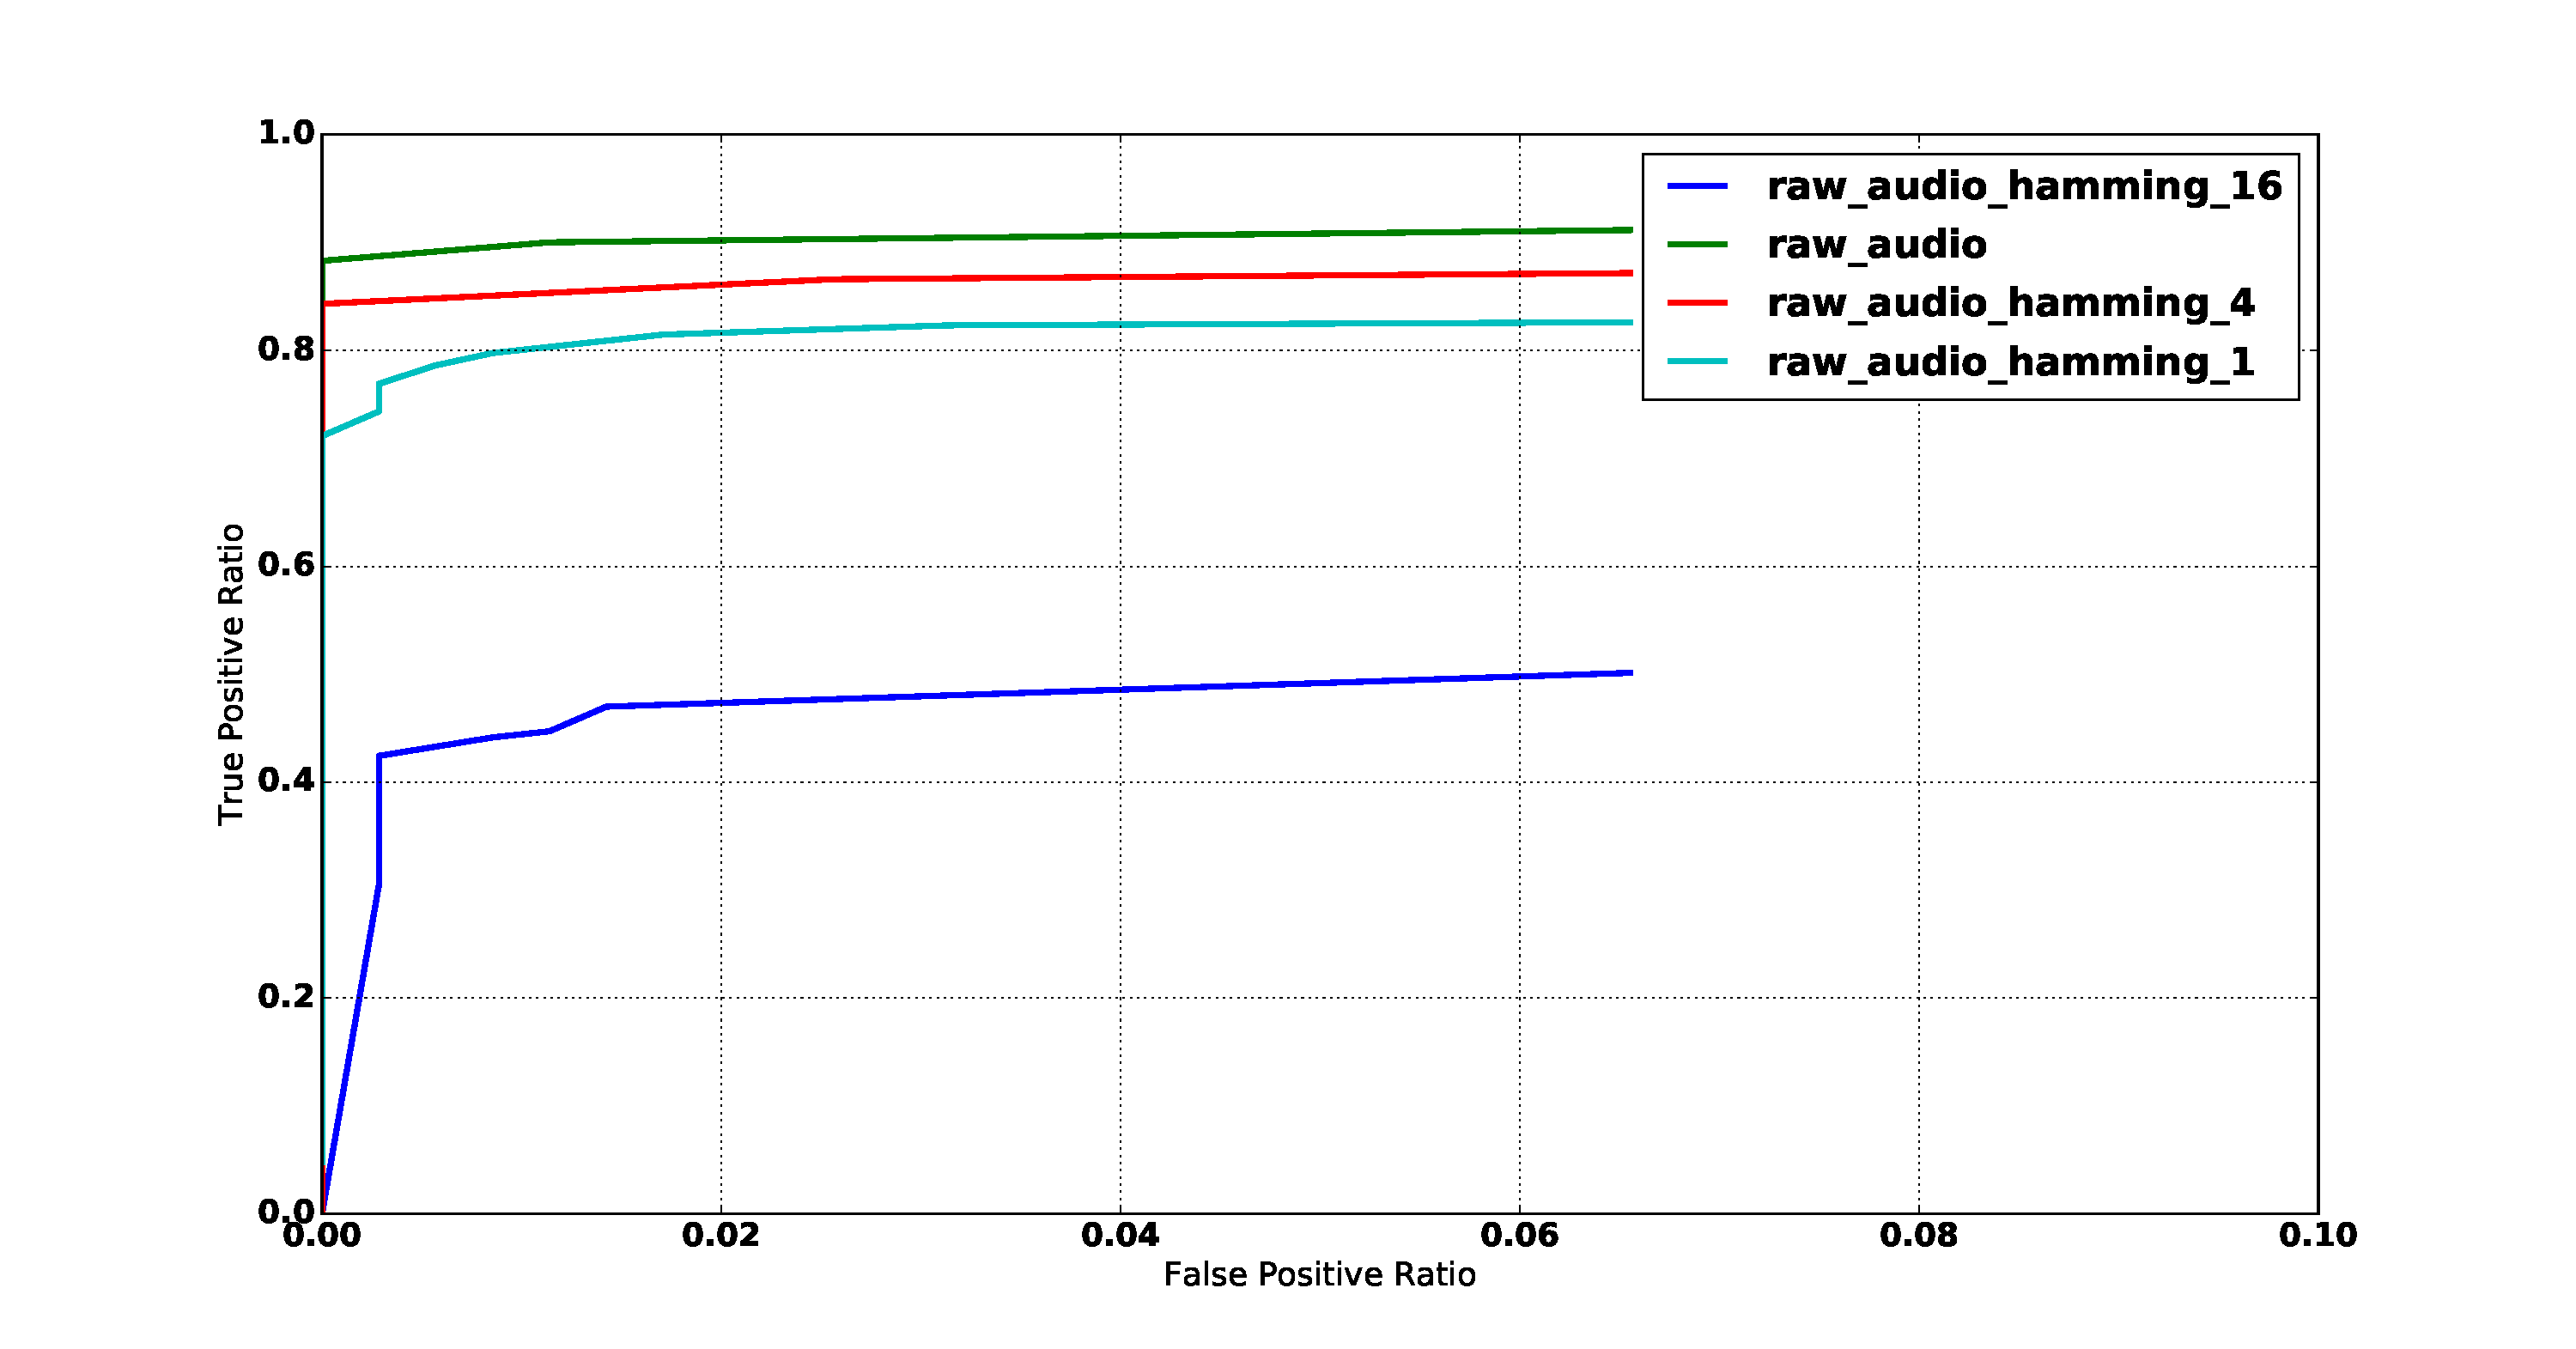
\includegraphics[width=\textwidth]{sound/roc_raw_audio.pdf}
\caption{Receiver Operating Curve (ROC) for Keyphrase Recognition on Raw Audio and Raw Audio obfuscated with Hamming Reduction}
\label{fig:roc_raw_audio}
\end{figure}



\begin{figure}[!th]
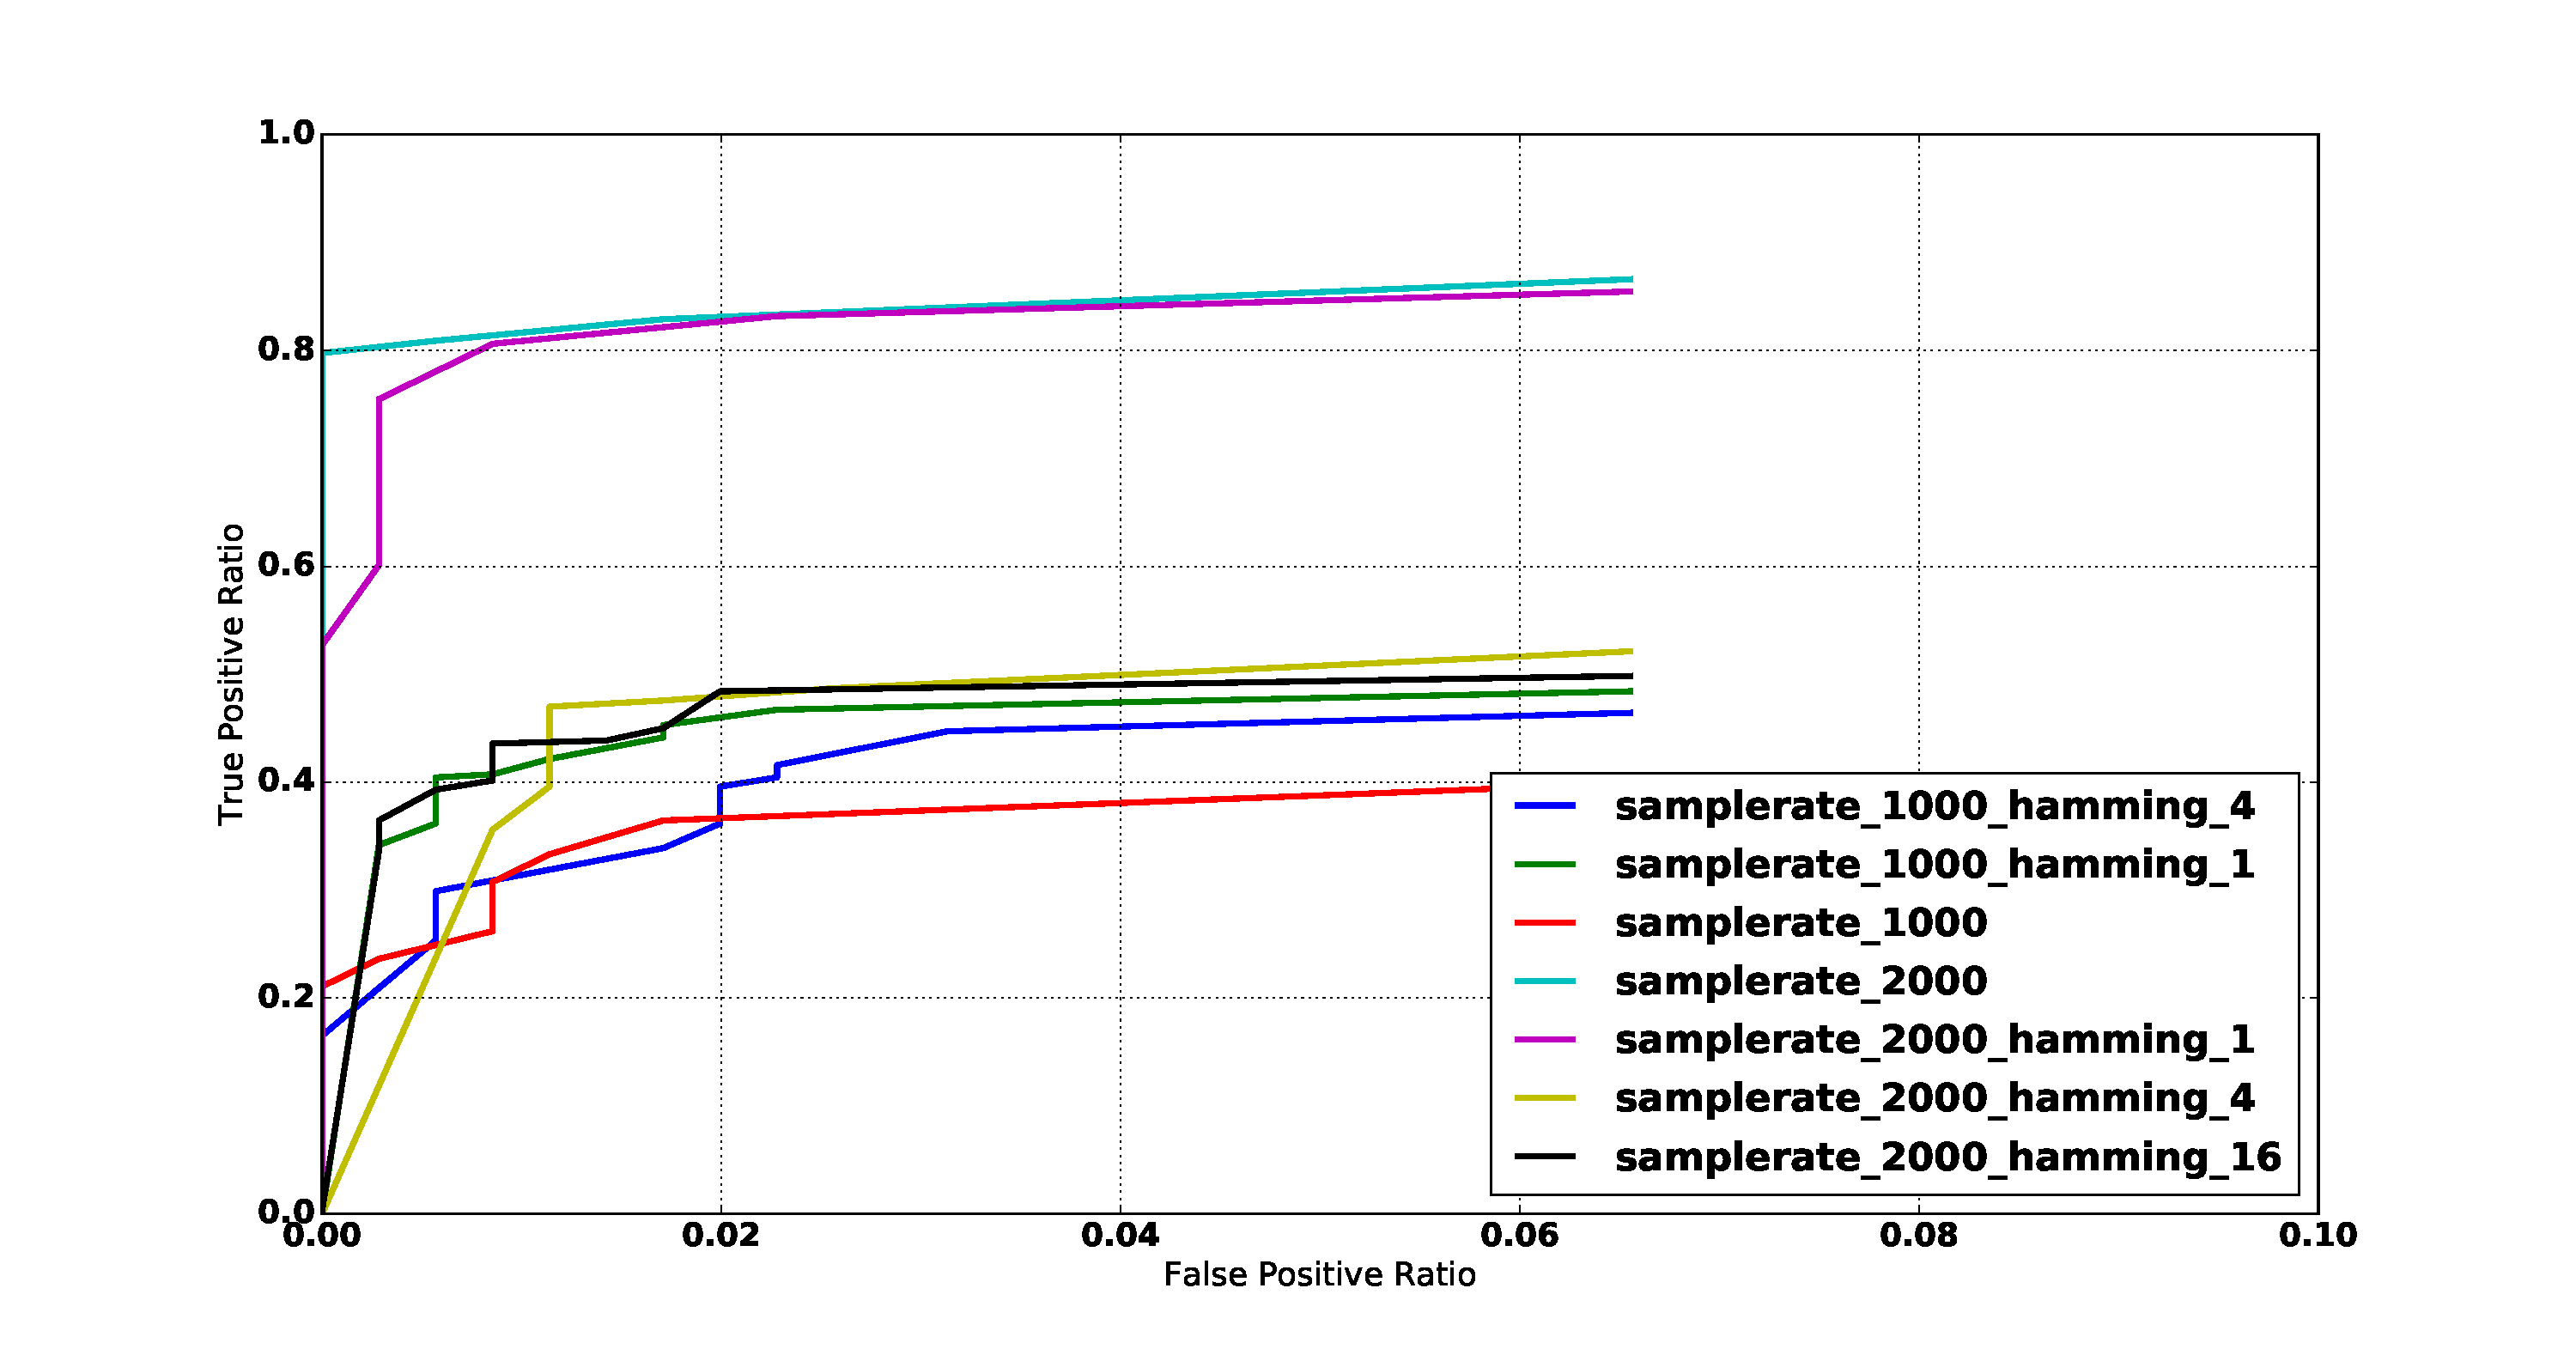
\includegraphics[width=\textwidth]{sound/roc_samplerate.pdf}
\caption{Receiver Operating Curve (ROC) for Keyphrase Recognition on Downsampled Audio and Downsampled Audio obfuscated with Hamming Reduction}
\label{fig:roc_samplerate}
\end{figure}



\begin{figure}[!th]
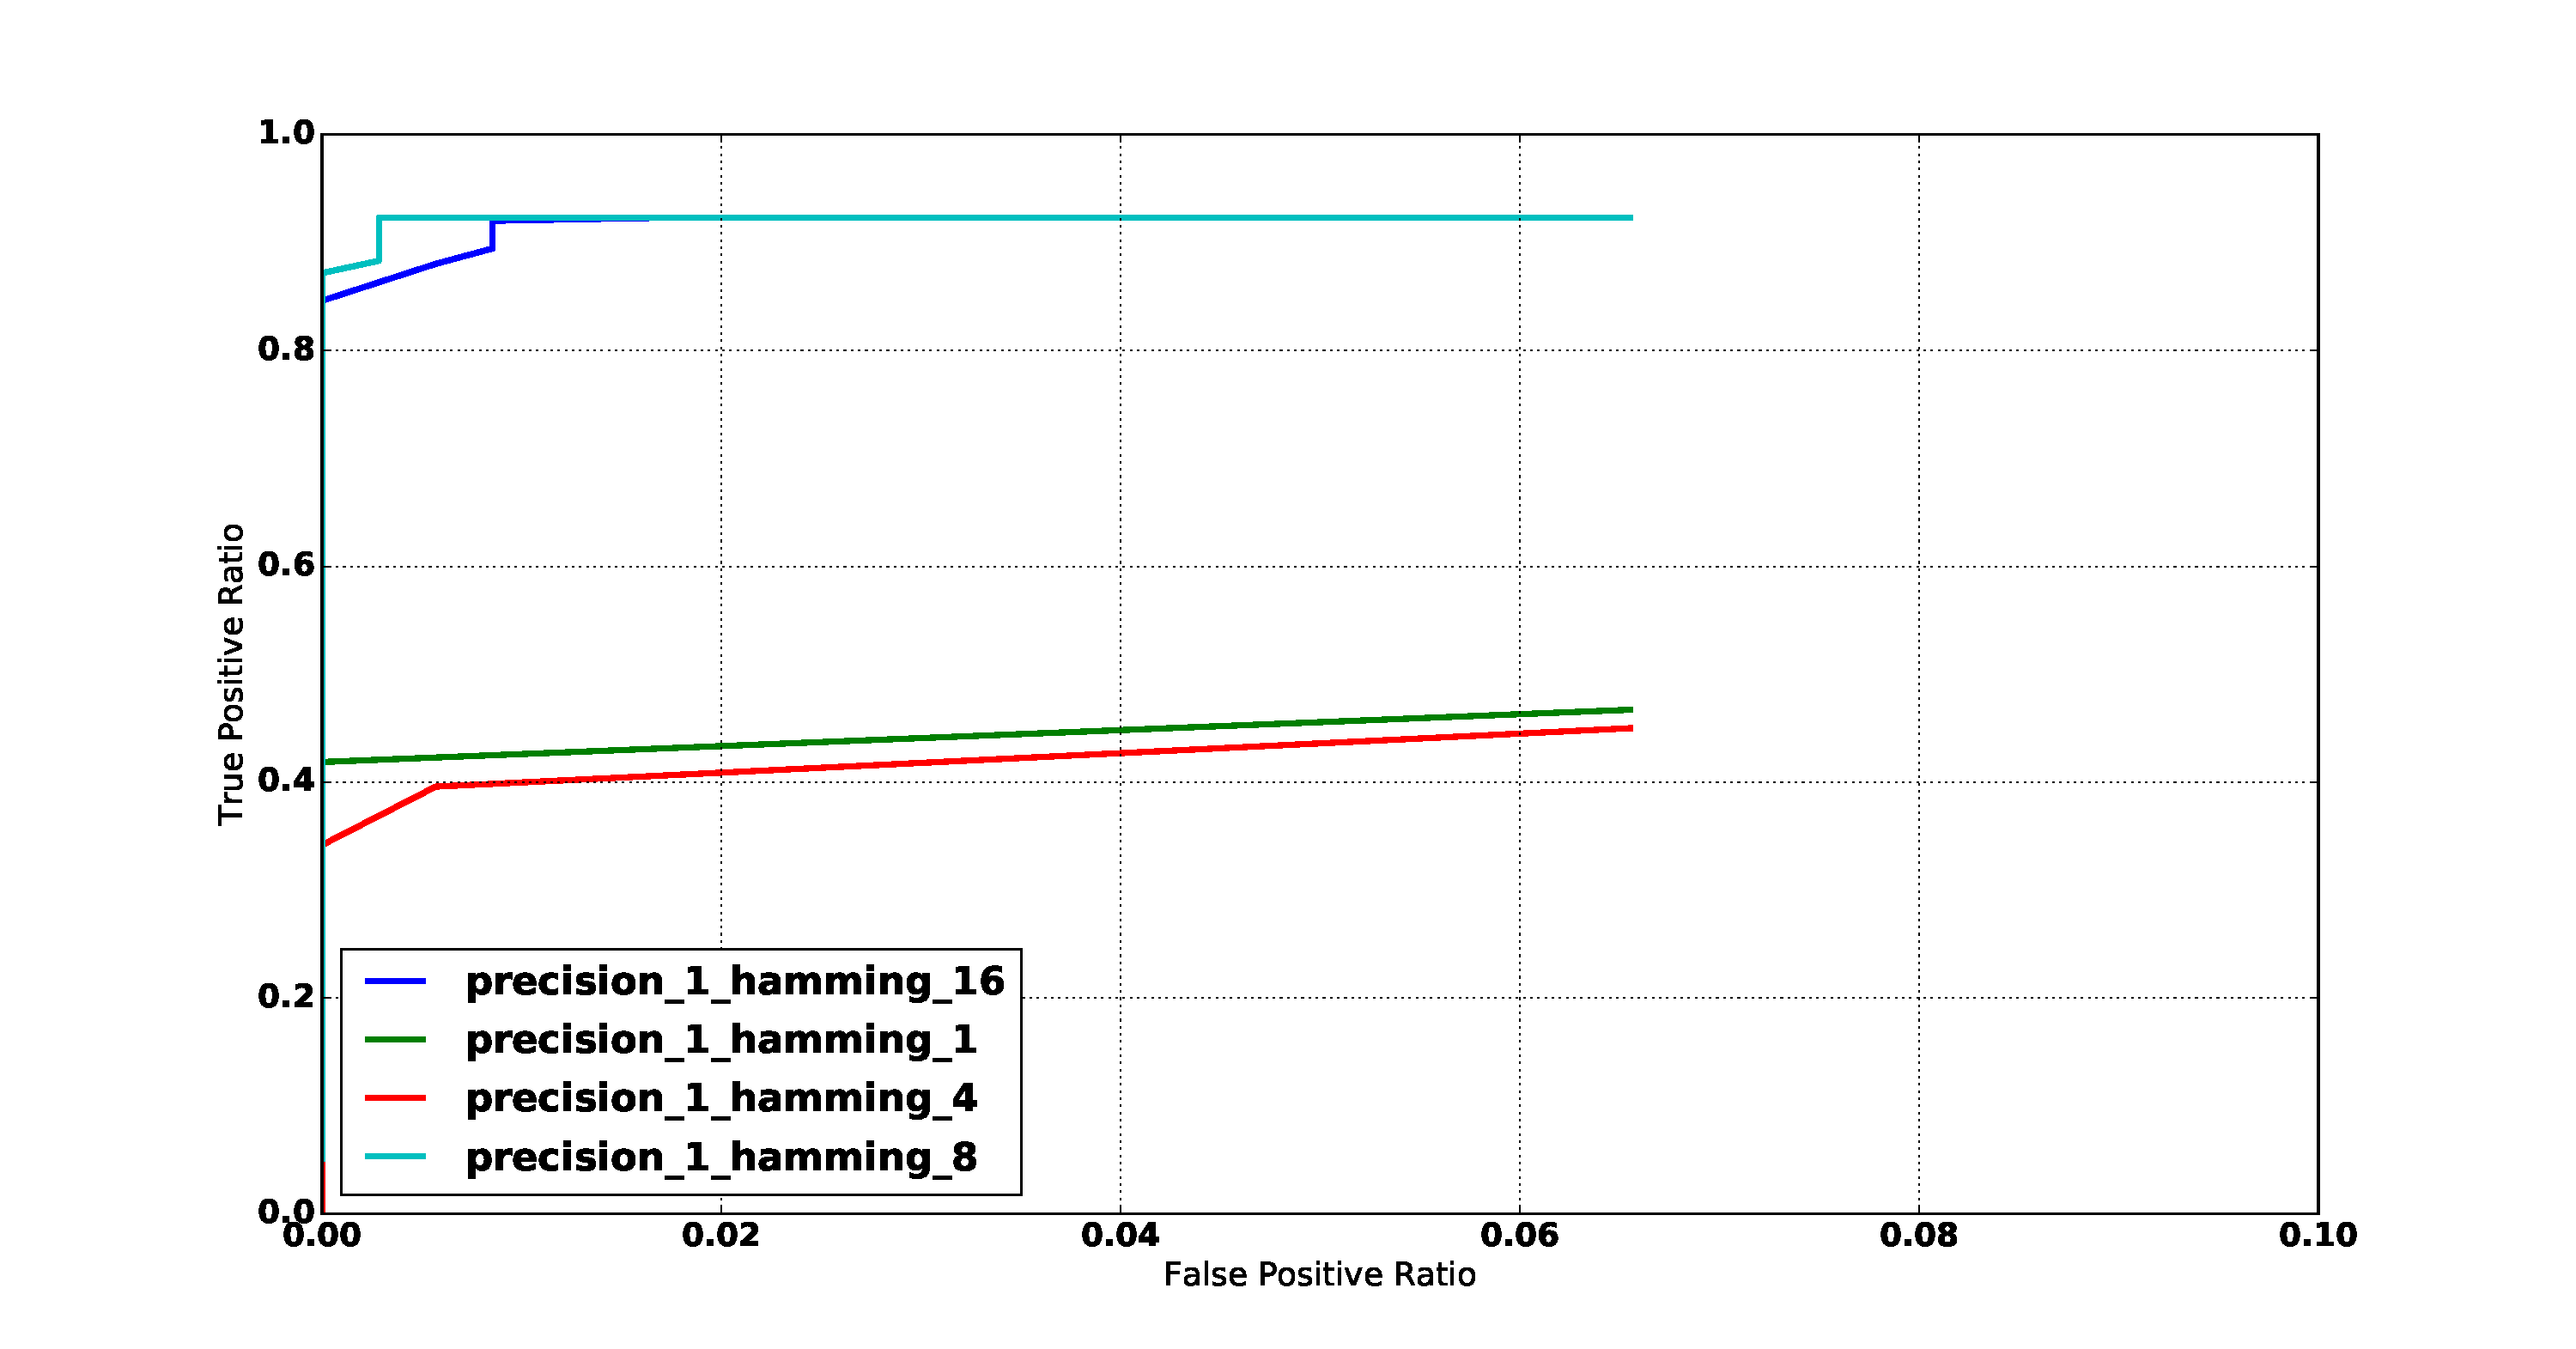
\includegraphics[width=\textwidth]{sound/roc_precision_bits.pdf}
\caption{Receiver Operating Curve (ROC) for Keyphrase Recognition on Low-precision Audio and Low-precision Audio obfuscated with Hamming Reduction}
\label{fig:roc_precision_bits}
\end{figure}




\section{Proposed changes to Mobile Keyphrase Recognition}
\label{sec:proposed_changes_to_mobile}

Using the obfuscated audio technique proposed by the results from the dbHound experimental evaluation, I propose that the Android sensor hub applies the obfuscation to microphone audio and broadcasts it to the applications on the device that wish to provide a voice command interface.
 This model is illustrated in Figure \ref{fig:proposed_voice_command_arch}.
 This way, applications such as browsers wishing to provide simple voice commands (such as "go back", "open new tab" etc.) will not infringe upon the privacy of the user.

\begin{figure}[!t]
\centering
\tikzset{%
    cascaded/.style={%
        general shadow={%
            shadow scale=1,
            shadow xshift=-1ex,
            shadow yshift=1ex,
            draw,
            thick,
            fill=white
        },
        general shadow={%
            shadow scale=1,
            shadow xshift=-.5ex,
            shadow yshift=.5ex,
            draw,
            thick,
            fill=white
        },
        fill=white,
        draw,
        thick,
        minimum width=1.5cm,
        minimum height=2cm
    }
}

\tikzstyle{vecArrowShort}=[thick,
                      shorten >= 5.5pt,
                      postaction={draw,line width=2pt, black, shorten >= 4.5pt}
]
\tikzstyle{vecArrow}=[thick,
                      postaction={draw,line width=2pt, black}
]

\tikzstyle{shortline} = [draw, -latex', fill=black, vecArrowShort]
\tikzstyle{line} = [draw, -latex', fill=black, vecArrow]
\tikzstyle{shortline2} = [draw, dotted, -latex', fill=black, vecArrowShort]
\tikzstyle{line2} = [draw, dotted, -latex', fill=black, vecArrow]

\tikzstyle{input} = [rectangle, draw, fill=green!20, text centered, sharp corners, minimum height=2em, minimum width=15em, align=center]
\tikzstyle{oper} = [rectangle, draw, fill=blue!20, text centered, rounded corners, minimum height=4em, minimum width=10em]
\tikzstyle{output} = [draw, ellipse,fill=red!20, minimum height=2em]

\begin{tikzpicture}[node distance = 2cm, auto]

% nodes
\node [input] (input) { $\text{Microphone}$ };
\node [oper, below of=input] (sensorhub) { $\text{Sensor Hub: Obfuscate Audio}$ };
\node [oper, right of=sensorhub, node distance = 8cm] (dbhound) { $\text{dbHound App}$ };
\node [cascaded, output, below of=sensorhub] (apps) { $\text{Client Applications}$ };

%arrows
\path [line] (input) -- (sensorhub);
\path [line2] (input) -- (dbhound);
\path [shortline] (sensorhub) -- (apps);
\path [shortline2] (dbhound) -- (apps);

\end{tikzpicture}
\caption{Proposed Voice Command Model for Mobile Systems showing dbHound equivalent in parallel}
\label{fig:proposed_voice_command_arch}
\end{figure}



\section{Conclusion}


In this chapter, I present the dbHound system in detail and discuss lightweight obfuscation techniques that can be implemented on mobile devices.
 Based on the experimental data, the most promising obfuscation technique is \texttt{precision\_1\_hamming\_16}.
 In other words, reducing the audio to 1-bit precision and applying the hamming reduce operation over 16 consecutive samples shows the best trade-off between privacy and keyphrase recognition performance.


I envision that such voice-recognition models based on obfuscated audio will provide the solution to maintaining user privacy while improving the accessibility of technology for the physically challenged, as well as providing users with an improved way of interfacing with technology.

\chapter{Conclusion}


%% etc, etc.

%% Do you have appendices?  If so, add them here, just like chapters.
% \begin{appendices}
% \include{backmatter/appendix1}
% \end{appendices}

%% Are you a big nerd with a colophon?  Add it here.
% \begin{colophon}
% \input{backmatter/colophon}
% \end{colophon}

%% McBride is a very nice style (some version is included in this distribution)
\bibliographystyle{mcbride}
\bibliography{refs/refs.bib,refs/hotmobile17refs.bib}

%% Want an index?  Neither did I.
%\printindex

\end{document}
